\documentclass[Lau, oneside, noexaminfo]{sapthesis}%remove "english" for a thesis written in Italian
\graphicspath{ {images/} }
%Bachelor's (laurea triennale) thesis : Lau 
%Master's (laurea specialistica) thesis: LaM 
%PhD's thesis: PhD 
\usepackage[italian]{babel} %use this package for a thesis written in Italian
\usepackage[T1]{fontenc}
\usepackage[utf8]{inputenx}
\usepackage{listings}
\usepackage{hyperref}
\usepackage{wrapfig}
\usepackage{float}
\usepackage{lettrine}
\usepackage{subcaption}
\usepackage{bookmark}
\usepackage{color}
%portare linespread a 1.1-1.3
\linespread{1.3}
%\usepackage{chngcntr}
\usepackage[nottoc, notlof, notlot]{tocbibind}
\usepackage{selinput}
\SelectInputMappings{
	agrave={à},
	eacute={é},
	Euro={€},
	accent={ ̀}
}
%\onehalfspacing
%\counterwithout{footnote}{chapter}

\usepackage{hyperref}
\hypersetup{
	hyperfootnotes=true,			
	bookmarks=true,			
	colorlinks=true,
	linkcolor=red,
    linktoc=page,
	anchorcolor=black,
	citecolor=red,
	urlcolor=blue,
	pdftitle={Sviluppo App},
	pdfauthor={Edoardo Gabrielli},
	pdfkeywords={thesis, sapienza, roma, university}
}

\definecolor{lightgray}{rgb}{.9,.9,.9}
\definecolor{darkgray}{rgb}{.4,.4,.4}
\definecolor{purple}{rgb}{0.65, 0.12, 0.82}

\lstdefinelanguage{JavaScript}{
  keywords={typeof, new, true, false, catch, function, return, null, catch, switch, var, if, in, while, do, else, case, break},
  keywordstyle=\color{blue}\bfseries,
  ndkeywords={class, export, boolean, throw, implements, import, this},
  ndkeywordstyle=\color{darkgray}\bfseries,
  identifierstyle=\color{black},
  sensitive=false,
  comment=[l]{//},
  morecomment=[s]{/*}{*/},
  commentstyle=\color{purple}\ttfamily,
  stringstyle=\color{red}\ttfamily,
  morestring=[b]',
  morestring=[b]"
}

\lstset{
   language=JavaScript,
   backgroundcolor=\color{lightgray},
   extendedchars=true,
   basicstyle=\tiny\ttfamily,
   showstringspaces=false,
   showspaces=false,
   numbers=left,
   numberstyle=\footnotesize,
   numbersep=9pt,
   tabsize=2,
   breaklines=true,
   showtabs=false,
   captionpos=b
}

\title{Progettazione e sviluppo della funzionalità di apertura di un verbale in InfoProf}
\author{Edoardo Gabrielli}
\IDnumber{1693726}
\course[]{Informatica}
\courseorganizer{Facolt\`a di Ingegneria dell'Informazione, Informatica e Statistica}
\submitdate{2019/2020}
\copyyear{2020}
\advisor{Prof. Emanuele Panizzi}
\authoremail{gabrielli.1693726@studenti.uniroma1.it}
\examdate{23 marzo 2020}
\examiner{Prof.}

%we refer to http://ctan.mirrorcatalogs.com/macros/latex/contrib/sapthesis/sapthesis-doc.pdf for an exhaustive description of the sapthesis documentclass.


\begin{document}

\frontmatter
\maketitle

\tableofcontents

\mainmatter
\chapter{Introduzione}
\label{ch:1}

\section{InfoStud e InfoProf}
\label{sec:pres}
L'app InfoStud nasce \textit{n} anni fa dalla necessità degli studenti di avere il sistema InfoStud sviluppato da InfoSapienza su mobile.
Data la natura poco \textit{mobile-friendly} del sistema web, nacque l'app ufficiale sotto il brand di SapienzaApps.

SapienzaApps, grazie al coordinamento del Prof. Emanuele Panizzi e all'aiuto degli studenti, pubblica e mantiene progetti come SeismoCloud, GeneroCity, InfoStud e InfoProf all'interno del Gamification Lab.

InfoStud è l'app che si rivolge unicamente agli studenti iscritti alla Sapienza e mette a disposizione un parco di funzionalità ampio che copre le funzioni standard del sistema padre (come visualizzazione e gestione esami) e andando oltre in alcuni casi: il sistema di gestione dell'orario didattico, la compilazione dei bollettini automatica, la prenotazione dei posti in biblioteca e molto altro.

InfoProf, al contrario, è l'app che si rivolge ai professori della Sapienza e vuole essere uno strumento alternativo, e più intuitivo, al sistema web. La ricerca della semplicità di utilizzo è la ricetta che accomuna tutti i progetti nel laboratorio ed ha bisogno di un'attenta progettazione per essere raggiunta. Spesso infatti ci si affeziona ad una interfaccia senza coglierne i problemi di usabilità. Ciò significa che bisogna sempre mettersi in discussione attraverso lo studio dei bisogni dell'utente, chiamato \textit{need finding}, la realizzazione di prototipi e il confronto con gli utenti finali tramite test di usabilità, con eventualmente molteplici iterazioni.

Lo stato dell'arte è un'app che permette di verbalizzare i voti degli studenti, attivare gli OPIS e cercare le aule. Queste funzionalità hanno un denominatore in comune: sono casi d'uso in cui l'utente potrebbe non avere il computer quando ha bisogno di utilizzarle. La verbalizzazione infatti può essere fatta subito dopo un orale, senza dover aspettare di tornare in ufficio e registrare i voti di tutti gli studenti. L'OPIS, date le ultime disposizioni, deve essere attivato durante la lezione, ma un utente potrebbe non voler portare un computer in aula solo per attivare il codice OPIS.

Il mio tirocinio è stato caratterizzato dall'aggiunta di piccole funzionalità richieste dall'utenza o dalla risoluzione dei bug: su InfoStud mi sono occupato di migliorare il login, aggiungere un'icona su SmartBiblio per indicare i posti non gestiti dal sistema, migliorare la dark-mode e aggiungere l'immagine del profilo degli studenti. Su InfoProf invece ho lavorato alla traduzione automatica, anche qui sul login, sul date-picker nella registrazione del voto di un esame e infine sul vero protagonista del tirocinio, ovvero l'apertura di un verbale, in cui ho fatto uno studio più approfondito di cui parlerò in \ref{ch:3}.

\section{Perché?}
\label{sec:why}
%trovare articoli scientifici in merito. 
Lo smartphone è ormai uno strumento radicato nella nostra quotidianità. Sono innumerevoli i modi in cui ha cambiato la nostra vita e la produttività è uno degli aspetti centrali. Nel settore pubblico l'evoluzione dei sistemi informatici però pecca di una rigorosa analisi progettazione, il che comporta perdite di tempo e difficoltà nell'utilizzo. Dall'indagine preliminare che ho svolto infatti emerge che alcuni intervistati trovano l'interfaccia web \textit{error-prone}, mentre un professore assunto recentemente, ha dichiarato che la piattaforma non è affatto user-friendly e che la logica vorrebbe che ci fosse un tasto "crea appello", non che debba andarlo a cercare in "verbalizzazione". Anche all'interno del team di sviluppo, quando ci è stata presentata per la prima volta l'interfaccia, abbiamo faticato a capire come svolgere i task che un professore è tenuto normalmente a fare. Tolti errori grossolani come l'assegnazione di termini differenti alla per rappresentare lo stesso concetto, esistono delle criticità che vanno contro la logica comune: se andiamo ad osservare la lista degli insegnamenti, alla destra di ogni elemento possiamo osservare un numero che rappresenta il numero di \textit{corsi} selezionati accoppiati con quell'insegnamento. Se selezioniamo il checkbox dell'elemento e andiamo all'interno del sotto-menù, deselezionando tutti i corsi, l'insegnamento rimarrà selezionato. Una buona interfaccia \textbf{(citare)}, invece, dovrebbe essere coerente e aiutare l'utente ad evitare gli errori.

%L'approccio che ho avuto quindi è stato quello di capire cosa gli utenti ritengono più importante nell'apertura di un verbale e mettere in secondo piano le funzionalità che vengono usate raramente. Vedremo infatti che paradossalmente l'interfaccia web, ai docenti che hanno imparato ad usarla, piace.

\chapter{Metodologie di sviluppo}
\label{ch:2}

\section{Organizzazione}
\label{sec:team}
Il team è composto da studenti impiegati nello sviluppo per circa tre mesi. La prassi è iniziare ad ambientarsi nei progetti attraverso l'attività di bug-fixing: familiarizzare con il codice e con i colleghi è centrale dato che per molti di noi è la prima esperienza all'interno di un progetto di tali dimensioni.

La metodologia di sviluppo che si adatta meglio alle nostre esigenze è l'Agile, il quale si basa su un insieme di regole il cui senso generale è un approccio adatto ai cambiamenti, non fisso e rigoroso, che misura i progressi attraverso codice funzionante e incoraggia il rilascio continuo del software per soddisfare l'utente finale. 

Un aspetto fondamentale che si ricollega a questo è l'integrazione continua del codice prodotto dagli sviluppatori: nel laboratorio utilizziamo GitLab, un sistema di controllo versione che tiene traccia delle modifiche, segnala i conflitti che possono generarsi dalla modifica simultanea dello stesso file e aiuta a gestire i compiti di ogni singolo sviluppatore.
Ad ogni \textit{merge request}, le modifiche apportate al codice sono revisionate da un controllo umano che garantisce la qualità del codice. Se infatti lo stile non è coerente con il resto del progetto, se ci sono bug introdotti dalle modifiche o altri problemi, la merge request viene respinta.

\section{Tecnologie utilizzate}
\label{sec:tech}
Per sviluppare il front-end delle applicazioni utilizziamo Ionic Framework v3, che è basato su AngularJS. Ionic permette di utilizzare tecnologie web per creare interfacce secondo gli standard di Android e iOS. Il vantaggio dell'uso di Angular è che il codice non va adattato ad alcuna piattaforma, inoltre per chiunque abbia già una discreta conoscenza della programmazione web, risulta abbastanza immediato iniziare a programmare. Tutto ciò velocizza molto la scrittura di una UI, ma bisogna fare dei compromessi: l'interfaccia non segue diligentemente gli standard imposti dal Material Design o dall'iOS UI Design perché deve adattarsi a entrambe le piattaforme. Un'altra criticità è che di fatto l'app è un'interfaccia web con caratteristiche \textit{app-like}, ovvero una Progressive Web App come Google le definisce. Questo spesso va a peggiorare significativamente le prestazioni. 
%Il ruolo di Ionic è fornire gli elementi dei vari standard di design già fatti e di integrare anche le funzionalità native attraverso Ionic Native o Cordova. Ciò significa che le prestazioni ne risentono ripetto ad un'app nativa. Inoltre ad oggi Ionic è alla versione 5, ma è impossibile aggiornare i progetti senza andare a creare dei conflitti che vanno risolti manualmente, vista la mole di codice che è stato scritto quindi, siamo costretti a rimanere ad una versione di qualche anno fa, all'occorenza programmando manualmente le novità introdotte dagli standard.

InfoStud ed InfoProf sono progettati seguendo un pattern architetturale simile ad MVC. L'idea generale è quella di tenere separate le responsabilità di ogni componente. Ciò si traduce sinteticamente in:

\begin{itemize}
	\item Model: rappresentano le classi, contengono i dati dell'applicazione a cui si accede attraverso i metodi che forniscono;
	\item View: la view accede ai dati forniti dai modelli e li presenta all'utente. Può comunicare con i controller, i provider e i model;
	\item Controller: il controller risponde alle azioni dell'utente intercettate dalla view e si occupa soltanto della logica di business, a volte comunica con i provider;
	\item Provider: di fatto "fornisce" i dati. Ha il compito di accedere alle API ed aggiornare i model.
\end{itemize}

\begin{figure}[H]
	\caption{Schema del funzionamento del pattern utilizzato da InfoStud e InfoProf.}
	\centering
	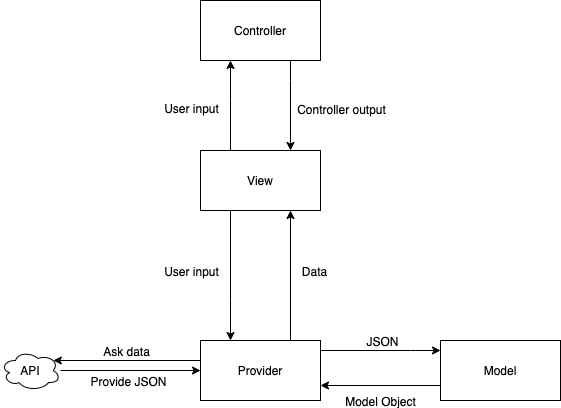
\includegraphics[width=0.8\textwidth]{arch-pattern-img}
	\label{fig:pattern}
\end{figure}

I vantaggi dell'utilizzo di questo modello è quello di separare la logica di presentazione, quella di business e quella di accesso ai dati in entità distinte tra loro in modo da favorire il lavoro di gruppo. Inoltre, essendo Angular un framework che impone una separazione in moduli del codice [citare], una divisione così fatta ne incoraggia il riuso.

%Tra ch 1 e 2 bisognerebbe aggiungere altre 8 pagine, magari apliare la descrizione delle issues

\chapter{Progettazione}
\label{ch:3}

L'attività di progettazione consiste nel trovare i bisogni dell'utente attraverso delle domande rivolte agli stessi, costruire un prototipo che rispecchi ciò che è emerso dalle risposte, eseguire dei test di usabilità sul prototipo e, a seconda delle criticità emerse dai test, modificare il prototipo e ripetere i test finchè si è trovata un'interfaccia che funzioni per gran parte degli utenti.

\section{Need-finding}
\label{sec:nf}
La prima cosa che ho fatto è capire quali sono i bisogni dell'utente. Non avendo mai utilizzato InfoStud docenti, il primo approccio al sistema è stato insieme al Prof. Panizzi che mi ha mostrato il processo di apertura di un verbale d'esame, le varie funzionalità già esistenti e i dati richiesti nel form che il docente è tenuto a compilare. Da questa dimostrazione sono emersi dei problemi: per un utente inesperto come me è difficile prendere confidenza con l'interfaccia in quanto, ad esempio, vengono utilizzati diversi termini per rappresentare lo stesso concetto, c'è una lista molto grande di insegnamenti da poter selezionare e bisogna prestare attenzione a quali sono quelli che si selezionano perché in alcuni casi il sistema potrebbe restituire un errore. Inoltre l'interfaccia non spiega come inserire il giorno dell'esame (quello che effettivamente gli studenti vedono in fase di prenotazione), bisogna chiederlo a chi già ne è a conoscenza.

A partire da questa premessa, ho creato un sondaggio inviando via email le seguenti domande:

\begin{enumerate}
	\item Preferisce aprire un verbale unico o aprirne uno per ogni corso che tiene? 
	\item Trova confusionario il processo di apertura di un verbale? Perché?
	\item Quanto tempo prima dalla data dell'esame apre il verbale?
	\item Quanto tempo dà agli studenti per prenotarsi?
	\item E quanti giorni prima, dal giorno dell'esame, chiude le prenotazioni? 
\end{enumerate}

Il sondaggio ha solo una domanda aperta, tra l'altro opzionale, in quanto volevo renderlo molto corto in modo da aumentare le possibilità di risposta. Per coloro che, invece, avessero voluto dedicarmi più tempo ho chiesto di argomentare per avere risposte più complete. 
%La prima domanda è stata fatta per capire come gestiscono la lista degli insegnamenti: la lista sull'app infatti è difficile da gestire vista la sua lunghezza. Quindi se la maggior parte dei professori sceglie di selezionare tutto, potrei sintetizzarla in qualche modo. La seconda ha un carattere generale, che mira a scoprire qualcosa di più da parte dell'utente. Le domande dalla 3 alla 5 invece servono a capire se esistono dei vincoli nella scelta delle date per cercare di automatizzare il processo.

Gli intervistati sono 60, presi casualmente in vari dipartimenti dell'ateneo in modo di avere un campione più eterogeneo possibile. I professori che hanno invece risposto sono stati 19.

\subsection{Verbale unico o uno per ogni corso?}

Come vediamo dall'immagine \ref{fig:d-i} la maggioranza degli intervistati preferisce aprire un verbale per ogni insegnamento. Ricordo che "un insegnamento", nella tabella, corrisponde a tutti gli insegnamenti vecchi che hanno cambiato nome e per ognuno esistono due righe: una per l'anno accademico corrente ed una per quello precedente.

\begin{figure}[H]
	\caption{Grafico delle risposte date alla prima domanda.}
	\centering
	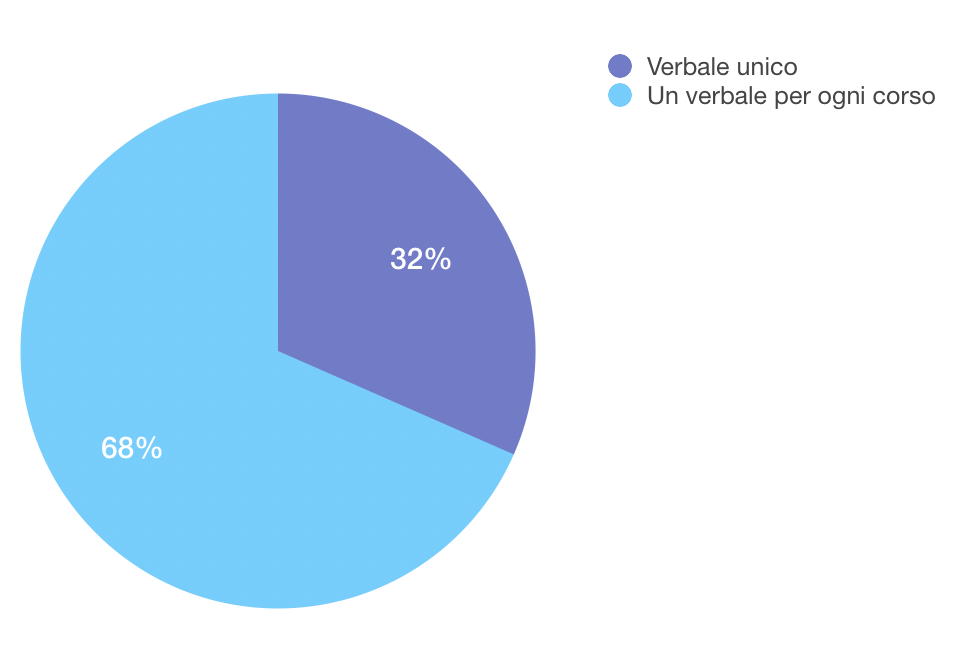
\includegraphics[width=0.6\textwidth]{d-i.png}
	\label{fig:d-i}
\end{figure}

\subsection{Trova confusionario il processo di apertura di un verbale?}
Qui i risultati sono un po' sorprendenti perché la maggioranza sostiene di non avere problemi, sebbene comunque una percentuale non trascurabile abbia risposto il contrario. Ciò potrebbe essere imputabile al fatto che per molti anni gli utenti sono stati abituati a questo sistema ed hanno imparato ad utilizzarlo agevolmente, con degli escamotage. Uno fra tutti è quello di utilizzare la funzionalità del "Duplica appello", che di fatto copia un verbale creato in precedenza portandosi dietro tutte le informazioni già compilate.

Inoltre alcuni dei docenti che hanno risposto "no" alla domanda, si sono espressi anche sul perché. Cito: 
\begin{itemize}
	\item "Il processo di apertura di un verbale più che confusionario è piuttosto "error-prone" con campi che si riempiono automaticamente o campi che scompaiono quando si effettua una scelta da un menù a tendina."
	\item "Ho difficoltà a mettere gli appelli di esame perché non so mai per quali corsi debba essere valido l'esame. E sovente gli studenti non vedono l'appello o meglio alcuni lo vedono e altri no."
	\item "La scelta degli insegnamenti è caotica perché ci sono nomi ripetuti con diverse diciture e lo stesso codice (non parliamo poi dei corsi di studio associati, che non apro neppure); l'anno accademico non serve a niente e complica l'immissione anche perché crea il refresh dell'elenco materie; oltre ad "avvisi e note" bisognerebbe poter inserire il luogo dell'esame e l'orario o i vari appelli, se più d'uno."
	\item "Un problema che trovo riguarda la scelta dell'A.A di riferimento. Vorrei che non esistesse questa opzione."
\end{itemize}

Ho avuto inoltre la fortuna di intervistare un docente assunto recentemente, che mi ha esplicitamente detto che ha avuto grosse difficoltà nell'aprire il suo primo verbale. Nessuno gli ha spiegato come fare, e che quindi ha impiegato molto tempo a cercare le funzionalità che gli servivano.

\begin{figure}[H]
	\caption{Grafico delle risposte date alla seconda domanda.}
	\centering
	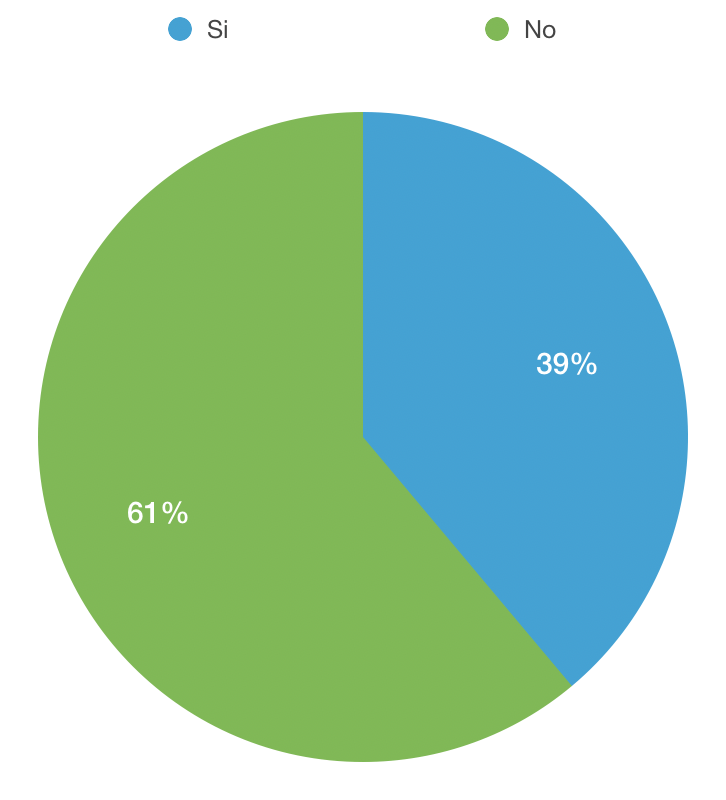
\includegraphics[width=0.4\textwidth]{d-ii}
	\label{fig:d-ii}
\end{figure}

\subsection{Quanto tempo prima dalla data dell'esame apre il verbale?}
La metà degli intervistati ha dichiarato di aprire i verbali all'inizio dell'anno accademico. Infatti da quello che ho potuto constatare, molti dipartimenti impongono questa condizione ai docenti, quindi è necessario velocizzare il tempo di apertura di un singolo verbale perché aprirne sette per ogni insegnamento potrebbe essere un'attività che porta via diverso tempo.

\begin{figure}[H]
	\caption{Grafico delle risposte date alla terza domanda.}
	\centering
	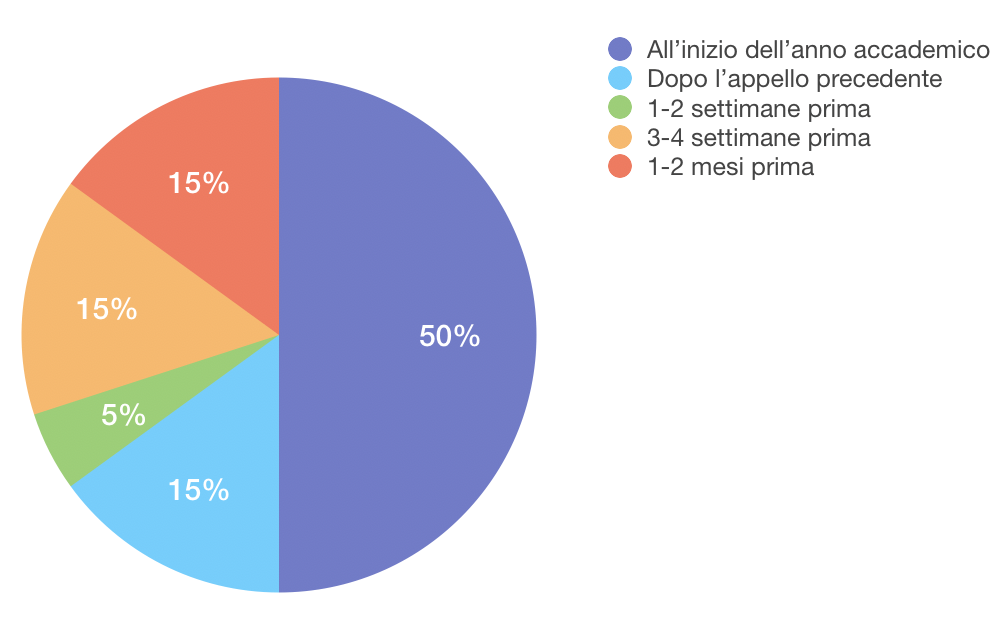
\includegraphics[width=0.8\textwidth]{d-iii}
	\label{fig:d-iii}
\end{figure}

\subsection{Quanto tempo dà agli studenti per prenotarsi?}
Qui le risposte sono piuttosto eterogenee.

\begin{figure}[H]
	\caption{Grafico delle risposte date alla quarta domanda.}
	\centering
	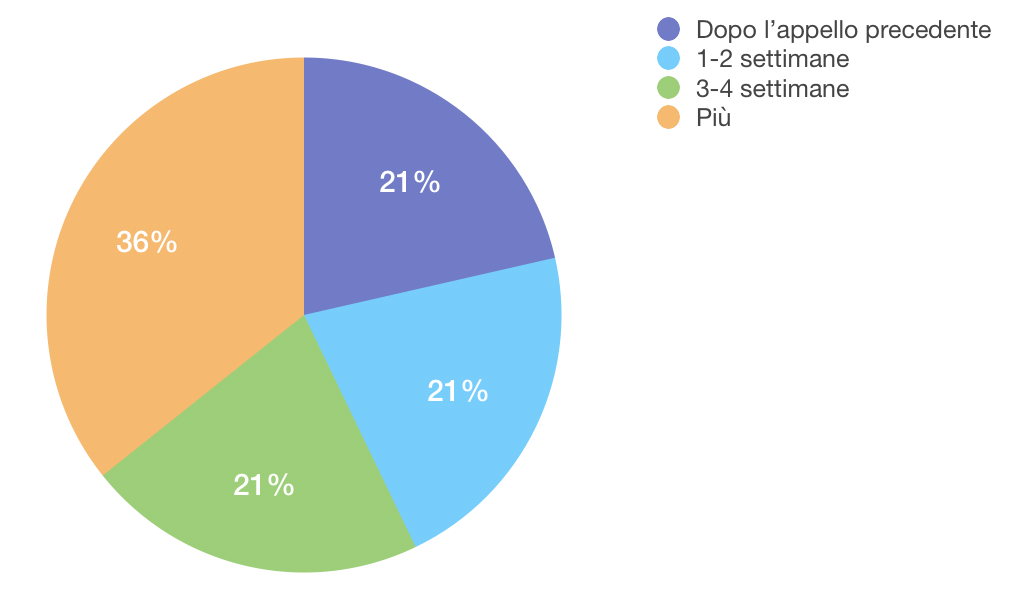
\includegraphics[width=0.8\textwidth]{d-iv}
	\label{fig:d-iv}
\end{figure}

\subsection{E quanti giorni prima, dal giorno dell'esame, chiude le prenotazioni?}
Al contrario qui la maggior parte dei docenti preferisce chiedere le prenotazioni uno o due giorni prima dal giorno dell'esame. 

\begin{figure}[H]
	\caption{Grafico delle risposte date alla quinta domanda.}
	\centering
	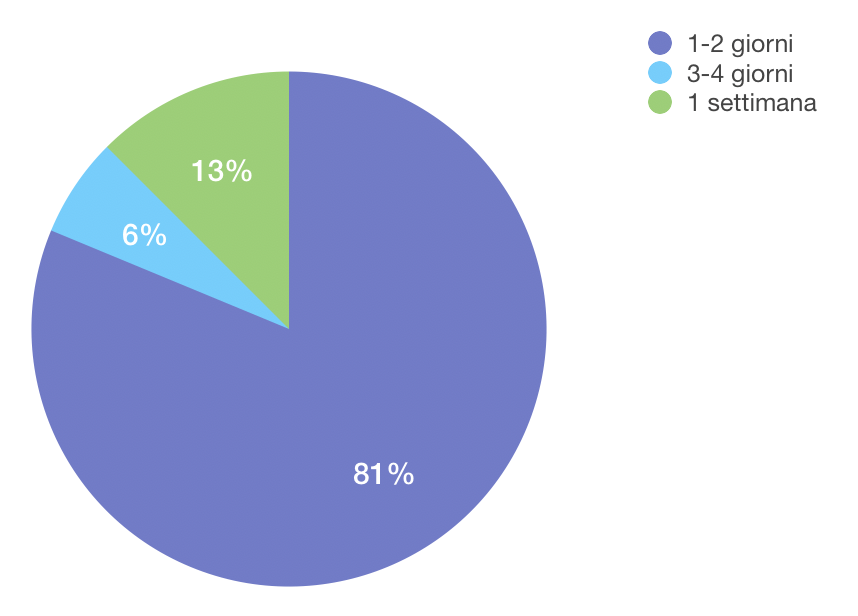
\includegraphics[width=0.7\textwidth]{d-v}
	\label{fig:d-v}
\end{figure}

\section{Requisiti}
\label{sec:req}
%citare "Developing SMASH", Nielsen e Gerhardt-Powals' cognitive engineering principles
Abbiamo visto che una buona percentuale dei partecipanti non è contenta dell'interfaccia desktop e mi ha dato degli spunti su cui lavorare, come l'aggiunta di orario e luogo d'esame. Inoltre sapere che diversi dipartimenti impongono l'apertura dei verbali ad inizio anno accademico è una delle motivazioni per cui è importante velocizzare il tempo di apertura di un verbale. Per raggiungere questo scopo ho pensato che una delle strade percorribili fosse quella di togliere un po' di informazioni su schermo e di non costringere l'utente a compilare tutti i campi del form. Dato che è impensabile eliminarli del tutto, si potrebbe creare un sistema di compilamento automatico e sintetizzare in qualche modo la tabella degli insegnamenti togliendo quegli elementi di ripetizione come l'anno accademico.

Dalle domande riguardanti le prenotazioni possiamo inoltre notare che, se da una parte le risposte sono state omogenee, per quanto riguarda invece il numero di giorni di prenotazione si osservano delle risposte molto frammentate. Quindi dare degli standard nella compilazione automatica (nel caso delle date) risulta essere poco coerente.

A partire dalle considerazioni fatte e dai problemi riscontrati sul sistema originale, ho stilato una lista di requisiti ad alto livello che guideranno tutte le iterazioni future:
\begin{enumerate}
	\item L'ambiente in cui l'app funzionerà per la maggior parte del tempo è su uno smartphone quindi, essendo uno schermo piccolo, è necessario togliere le informazioni superflue.
	\item L'apertura di un verbale deve avvenire nel minor tempo possibile, in modo da velocizzare l'apertura consecutiva di più verbali.
	\item L'interfaccia dovrebbe essere ragionevolmente semplice da capire ed utilizzare e senza aver bisogno di una spiegazione.
\end{enumerate}

\section{Iterazioni}
%parlare solo dei prototipi e fare una valutazione secondo test/euristiche a fine di ogni iterazione.
\subsection{Valutazione dell'interfaccia}
\label{heuristics}
%parlare di euristiche e test
Prima di cominciare a parlare della fase di prototyping, introduco le tecniche di valutazione che ho utilizzato. Queste tecniche testano l'usabilità e le funzionalità di un'interfaccia, in modo da valutare gli effetti che ha sull'utente ed eventualmente i problemi di usabilità. Per essere eseguite richiedono un artefatto che può essere sia un prototipo, che un implementazione completa. In questo caso procederò ad iterare su un prototipo nella fase iniziale, per poi implementarne direttamente le funzionalità applicando le tecniche di valutazione a fine di ogni iterazione.

Inizialmente ho valutato il prototipo attraverso dei test di usabilità "sul campo", con la partecipazione di rappresentati scelti a caso dagli utenti stessi. Essi prevedono di avere un prototipo funzionante da far provare agli utenti, i quali durante il test descrivono ciò che stanno facendo (think aloud). Nei casi in cui questo test produce poche informazioni ho introdotto la variante del \textit{cooperative evaluation} che permette sia all'utente che al valutatore di fare domandee. A causa di forza maggiore ho dovuto abbandonare questa via per fare spazio alle euristiche.

Le euristiche sono delle regole, o linee guida, utilizzate per valutare o guidare la progettazione delle interfacce grafiche. Per il mio progetto di tirocinio ho utilizzato le euristiche di Neilsen che riporto qui di seguito:
\begin{enumerate}
	\item Visibilità dello stato del sistema
	\item Corrispondenza tra il mondo reale e il sistema
	\item Libertà e controllo da parte degli utenti
	\item Coerenza e standard
	\item Prevenzione degli errori
	\item Riconoscere piuttosto che ricordare
	\item Flessibilit\'a ed efficienza d'uso 
	\item Design minimalista ed estetico
	\item Aiutare gli utenti a riconoscere, diagnosticare e correggere gli errori
	\item Aiutare e documentare
\end{enumerate}

\subsection{Iterazione 1}
L'apertura di un verbale è una delle funzionalità base del sistema InfoStud, per questo è importante che venga messa in prima pagina proprio dove viene mostrata la lista degli esami aperti in passato. Un bottone con il simbolo "+" in alto a destra suggerisce l'aggiunta di un nuovo elemento alla lista. Se cliccato, l'applicazione propone una la lista degli insegnamenti tenuti dal professore e un'altra di \textit{alias}. Gli alias sono etichette che si applicano ad uno o più insegnamenti in modo che se l'alias viene selezionato, allora vengono selezionati anche tutti gli insegnamenti ad esso collegati. Questo meccanismo va a sostituire quello che fa il "Duplica appello" di InfoStud desktop.

Inoltre accanto ad ogni insegnamento c'è un'icona blu "i" che se cliccata porta ad una nuova vista che mostra i corsi di studio in cui l'insegnamento è attivo. Questi elementi sono selezionabili e quando si clicca sul bottone "Continua" si arriva infine al form che richiede l'inserimento delle date di inizio e fine appello, inizio e fine prenotazioni, la necessità dell'OPIS ed eventualmente le note per gli studenti. La navigazione, così impostata, va a semplificare leggermente il form dividendolo in due pagine e quindi riducendo il carico di informazioni su una singola view. Il prototipo è visibile in figura \ref{fig:it-1}.

Un altro miglioramento che è stato apportato è quello del compilamento automatico delle date. L'idea è quella di selezionare la data di inizio dell'appello e l'app, ricordando le date che sono state utilizzate precedentemente, prevede quali saranno quelle che l'utente inserirà, facendolo per lui. Infatti se dalle interviste è emerso che i professori tendono a frammentarsi nel scegliere il numero di giorni dedicati all'appello e alle prenotazioni, d'altro canto la maggior parte è costante e utilizza sempre quelli. Dunque far ricordare all'applicazione le scelte fatte dall'utente in precedenza può essere una soluzione percorribile e dovrebbe velocizzare di molto l'apertura di un verbale. % aggiungere eventuali feedback dati dalla beta

Nei test, ogni intervistato è sempre riuscito ad aprire il verbale senza difficoltà nell'ordine di pochissimi minuti. C'era qualche incertezza nel campo note, dove "Note per gli studenti" veniva spesso confuso con un placeholder. In pochi si sono interessati del tasto "i" accanto agli insegnamenti. Inoltre non avere nel form un'indicazione delle scelte fatte dall'utente nel corso della navigazione può essere una fonte di errore, quindi serve un modo per mostrare all'utente le scelte fatte nel corso della navigazione.

\begin{figure}[H]
	\begin{subfigure}{0.6\textwidth}
	  \centering
	  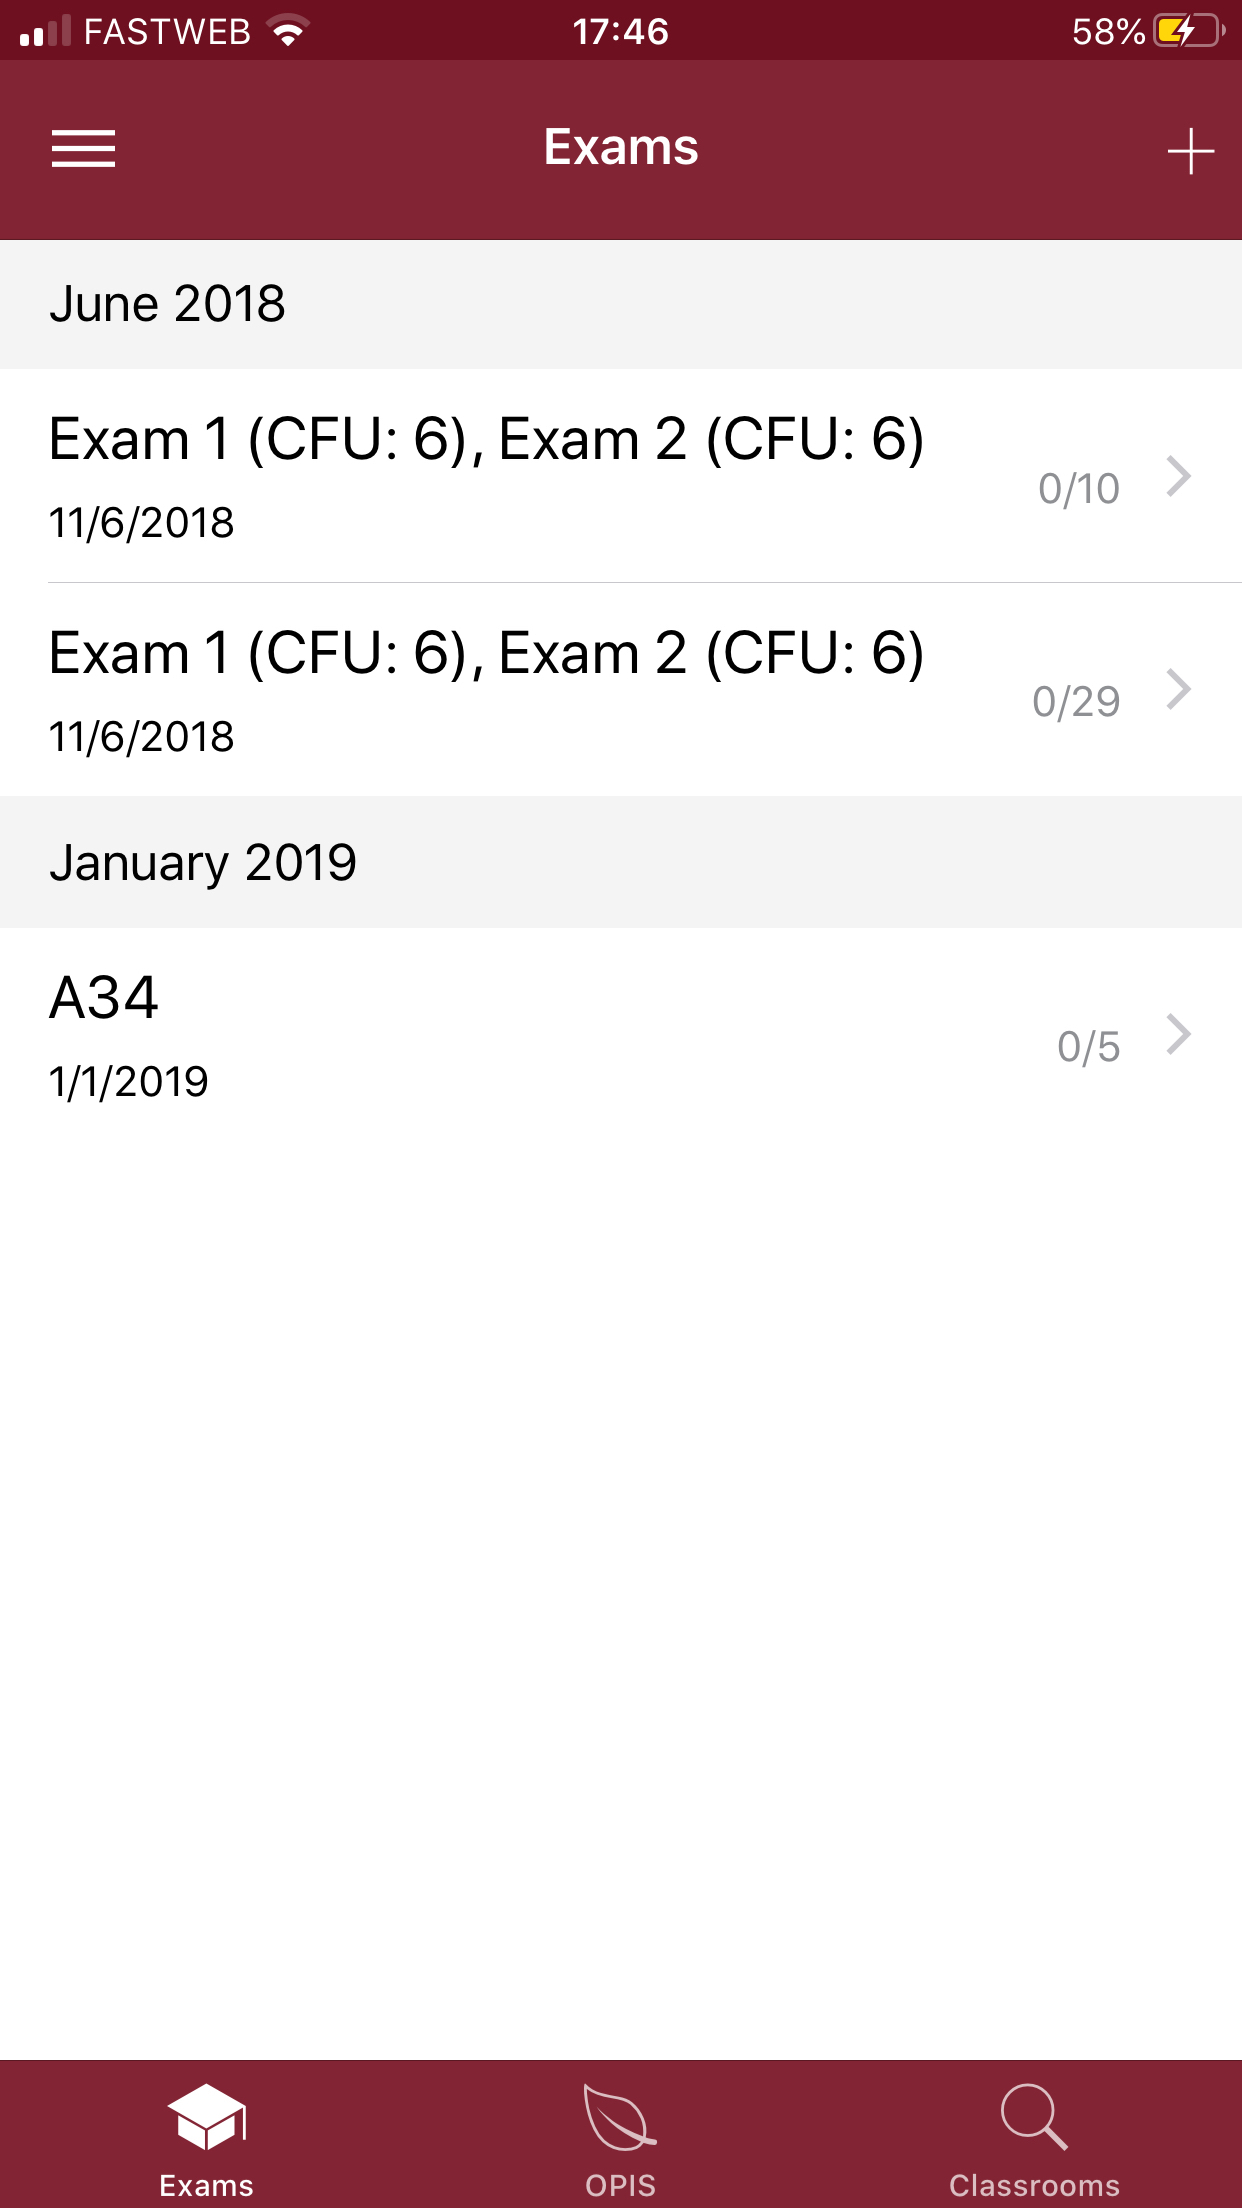
\includegraphics[width=0.5\linewidth]{ui-iterations/i/main}  
	  \caption{La prima pagina dell'applicazione InfoProf.}
	  \label{fig:sub-first}
	\end{subfigure}
	\begin{subfigure}{0.6\textwidth}
	  \centering
	  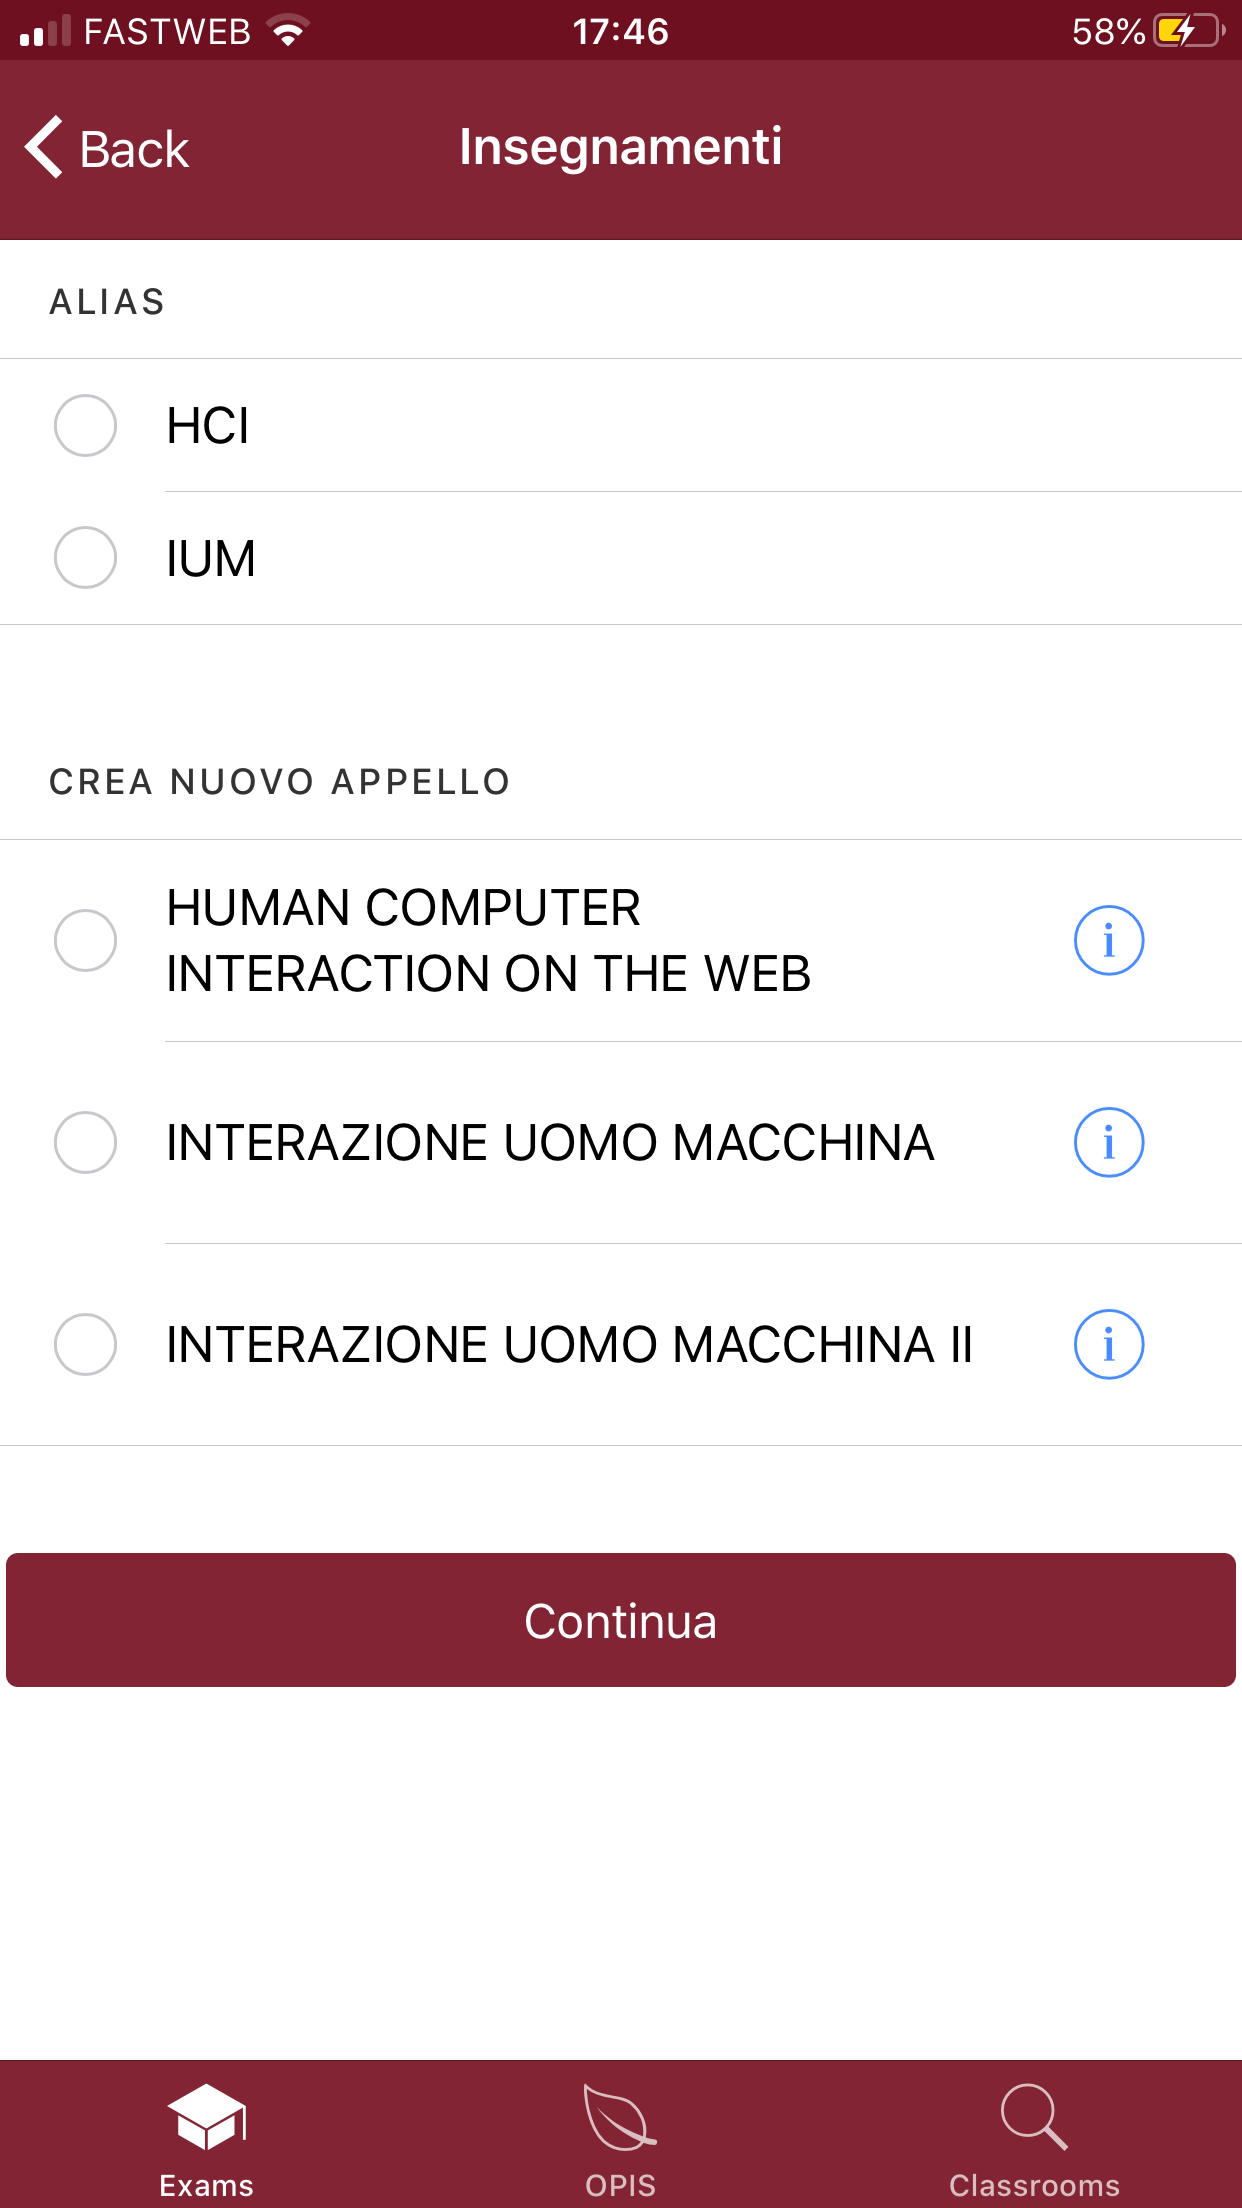
\includegraphics[width=0.5\linewidth]{ui-iterations/i/select-teaching}  
	  \caption{Pagina di selezione degli insegnamenti.}
	  \label{fig:sub-second}
	\end{subfigure}
	\begin{subfigure}{0.6\textwidth}
		\centering
		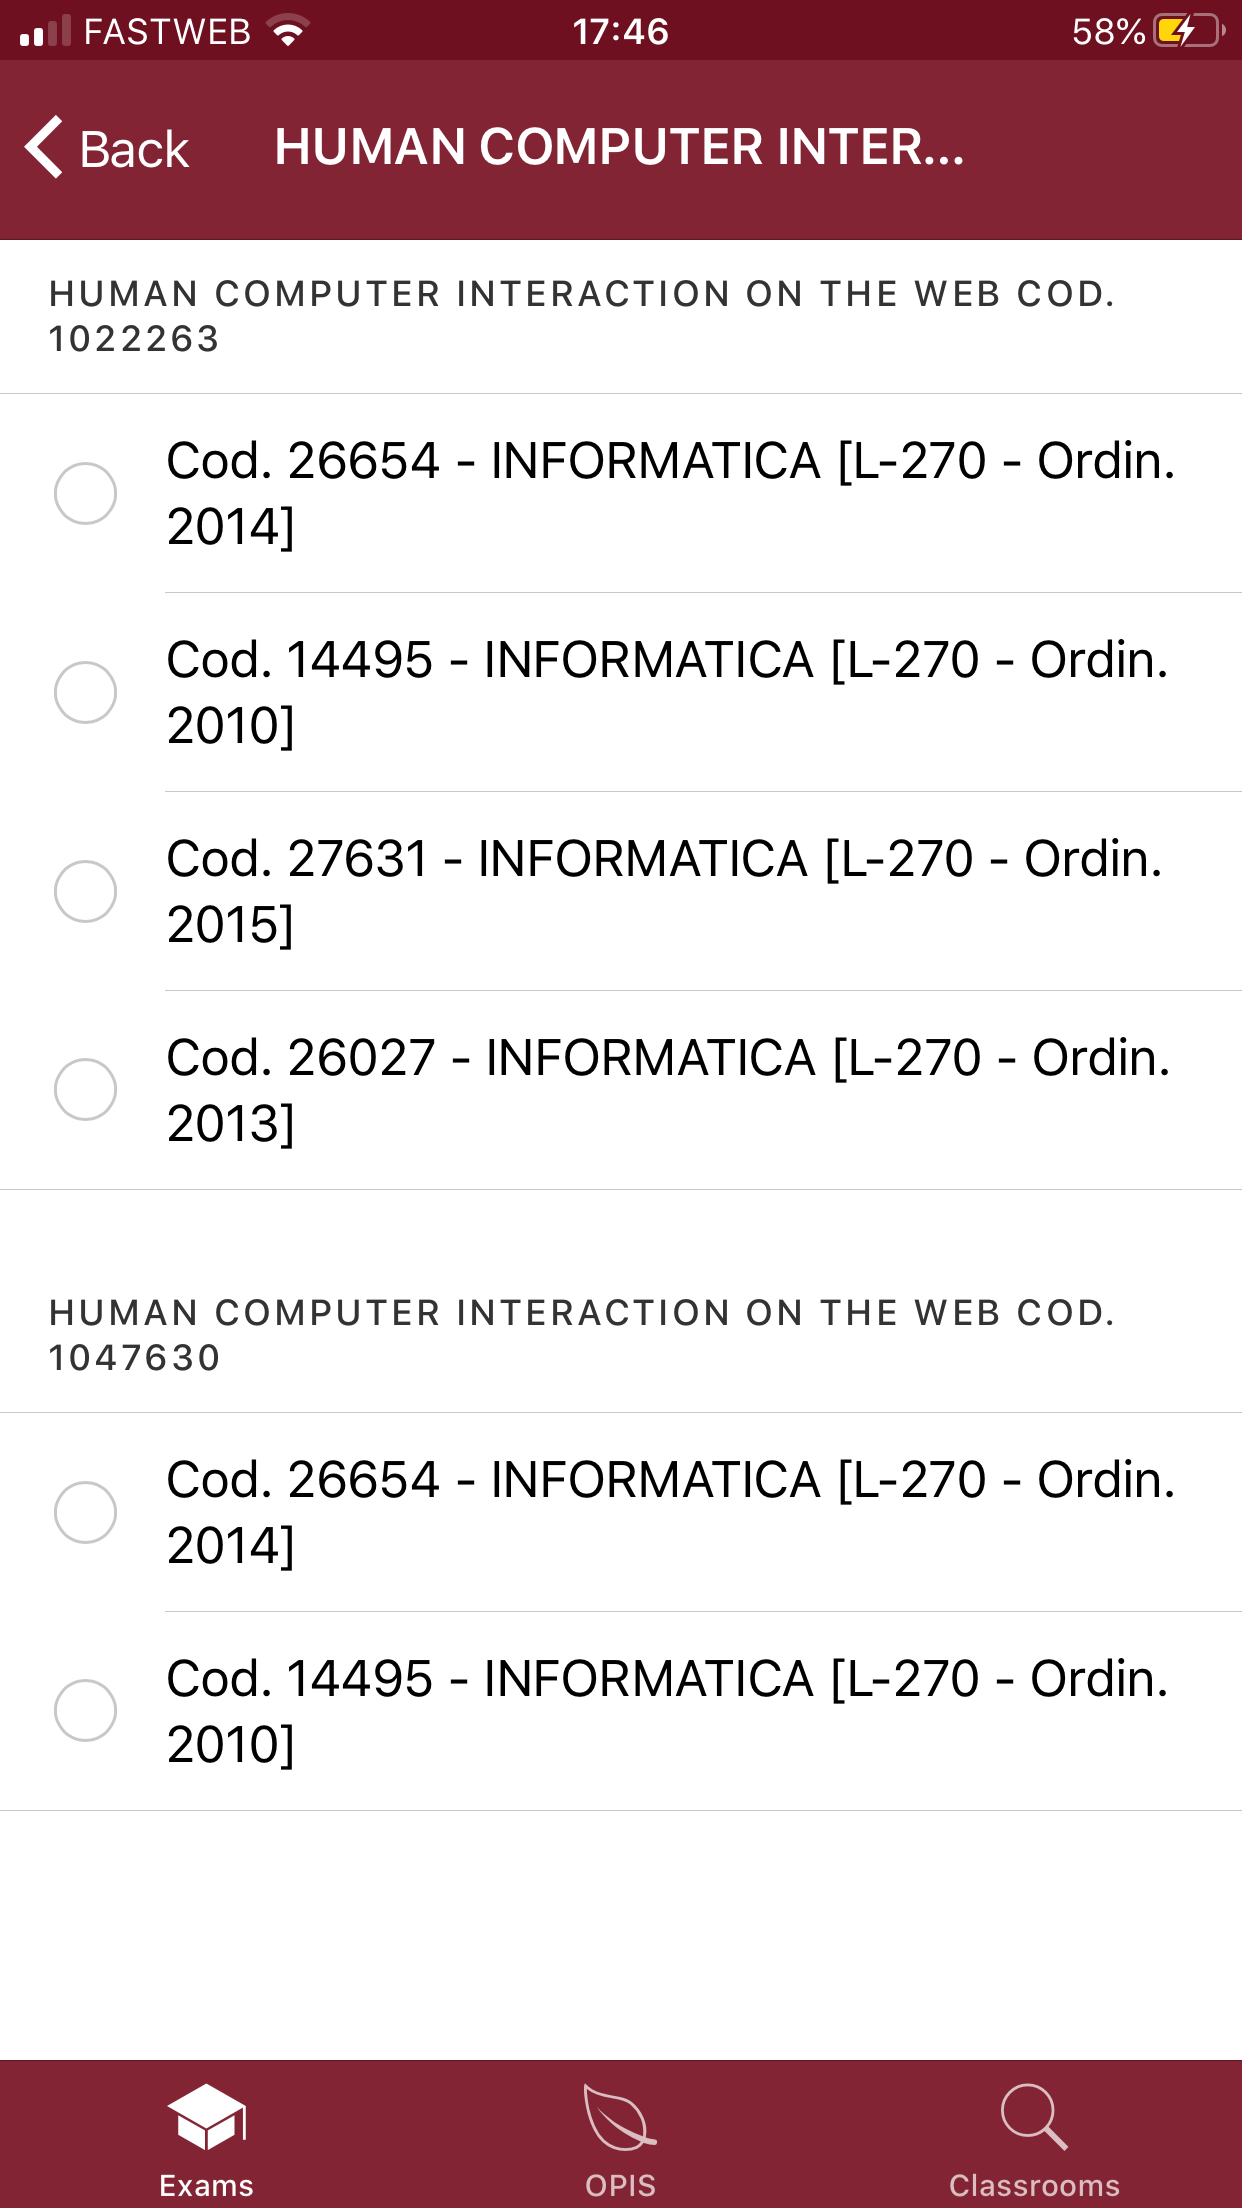
\includegraphics[width=0.5\linewidth]{ui-iterations/i/select-program}  
		\caption{Pagina per la selezione dei corsi di studio.}
		\label{fig:sub-third}
	  \end{subfigure}
	  \begin{subfigure}{0.6\textwidth}
		\centering
		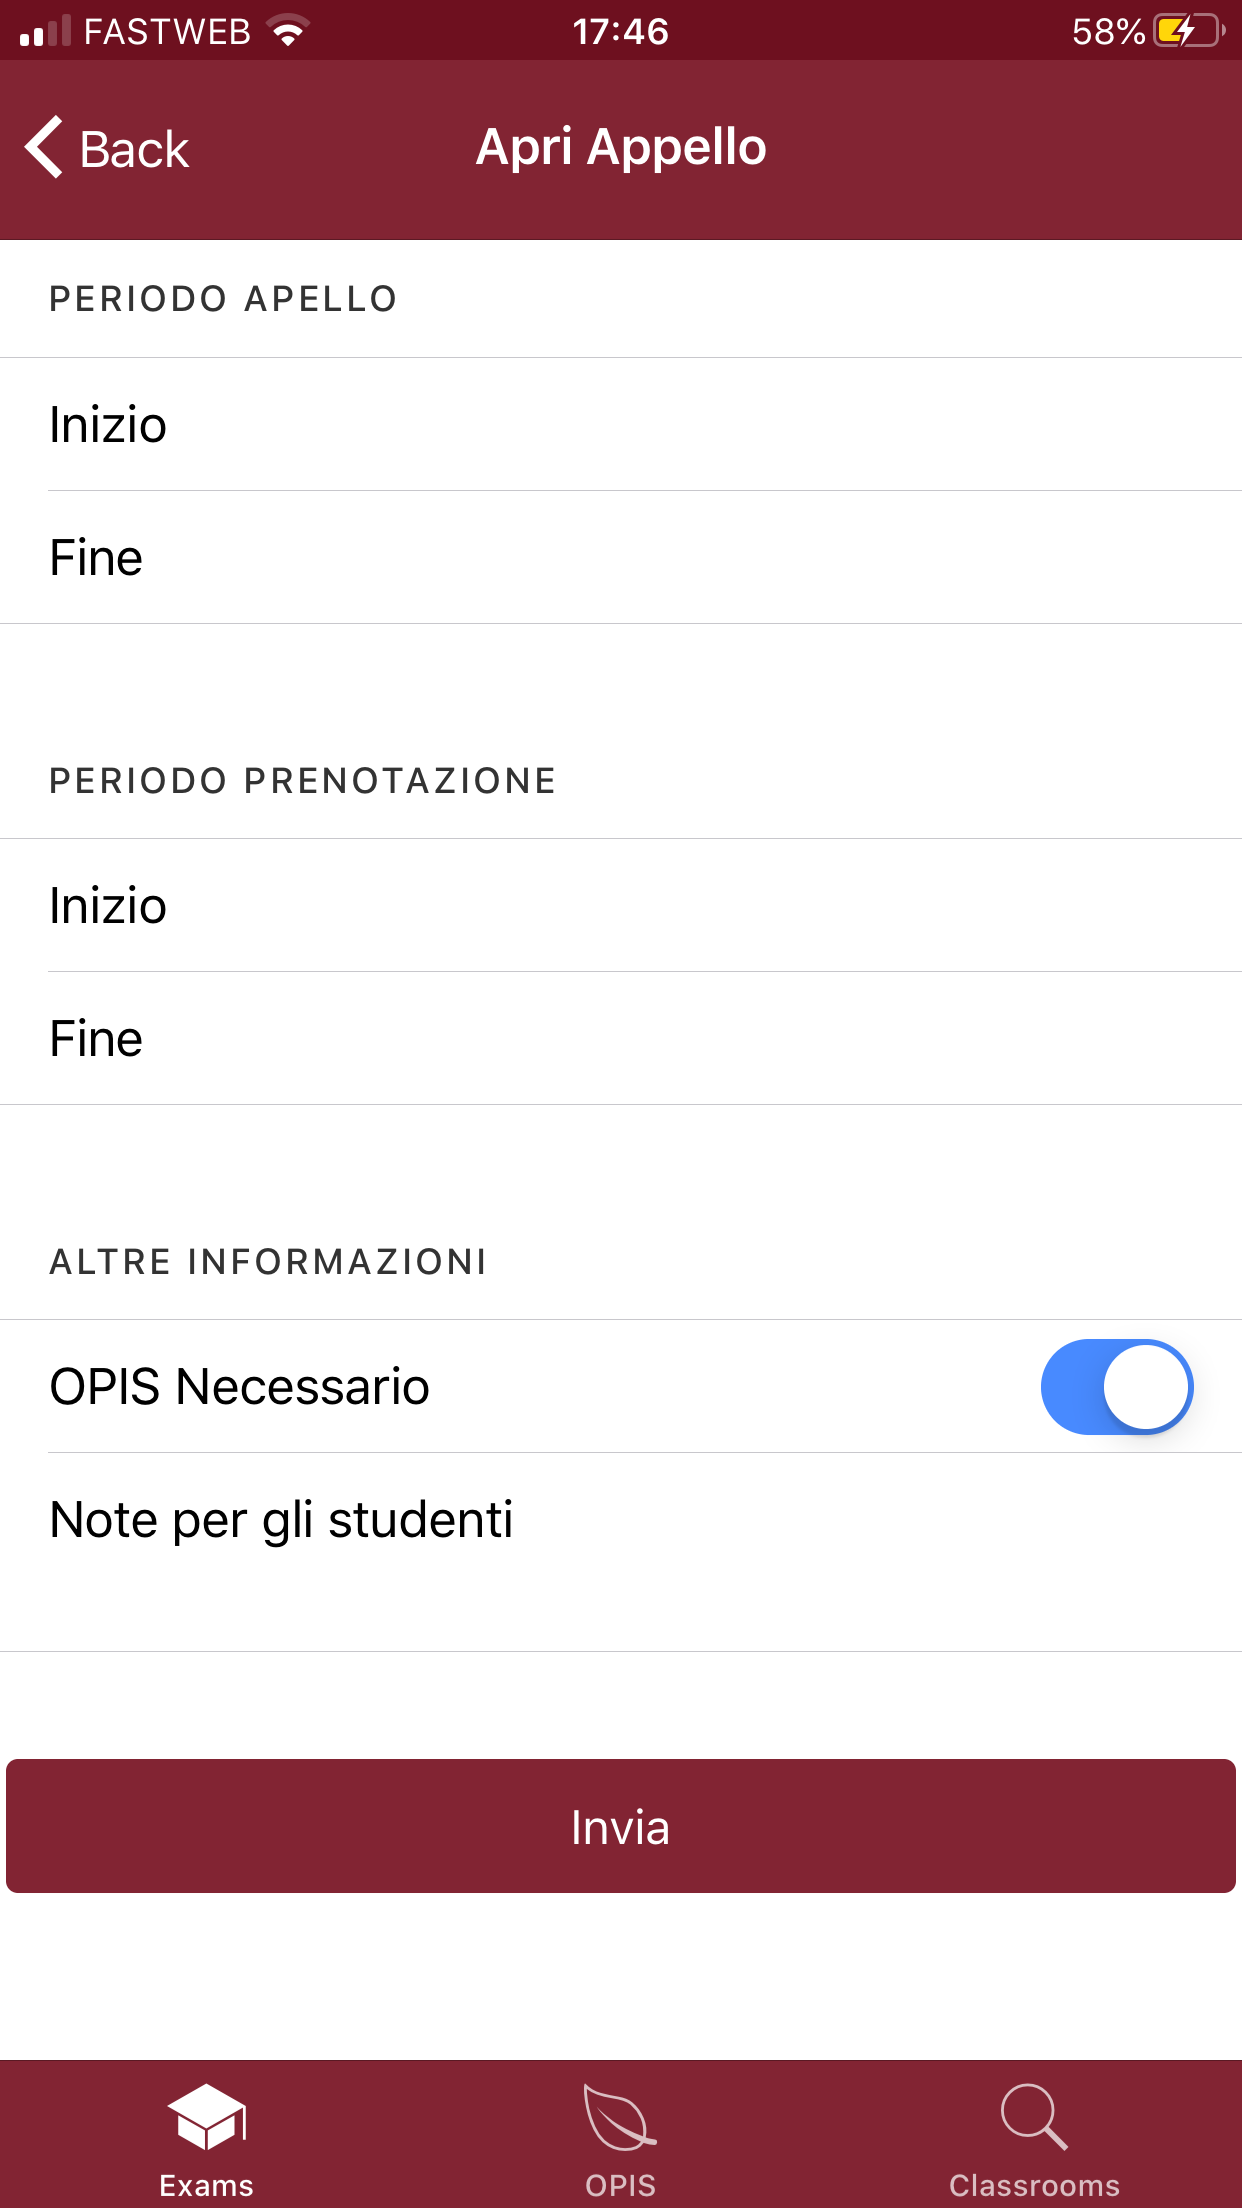
\includegraphics[width=0.5\linewidth]{ui-iterations/i/form}  
		\caption{Il form per inserire le informazioni del verbale.}
		\label{fig:sub-fourth}
	  \end{subfigure}
	  \begin{subfigure}{0.6\textwidth}
		\centering
		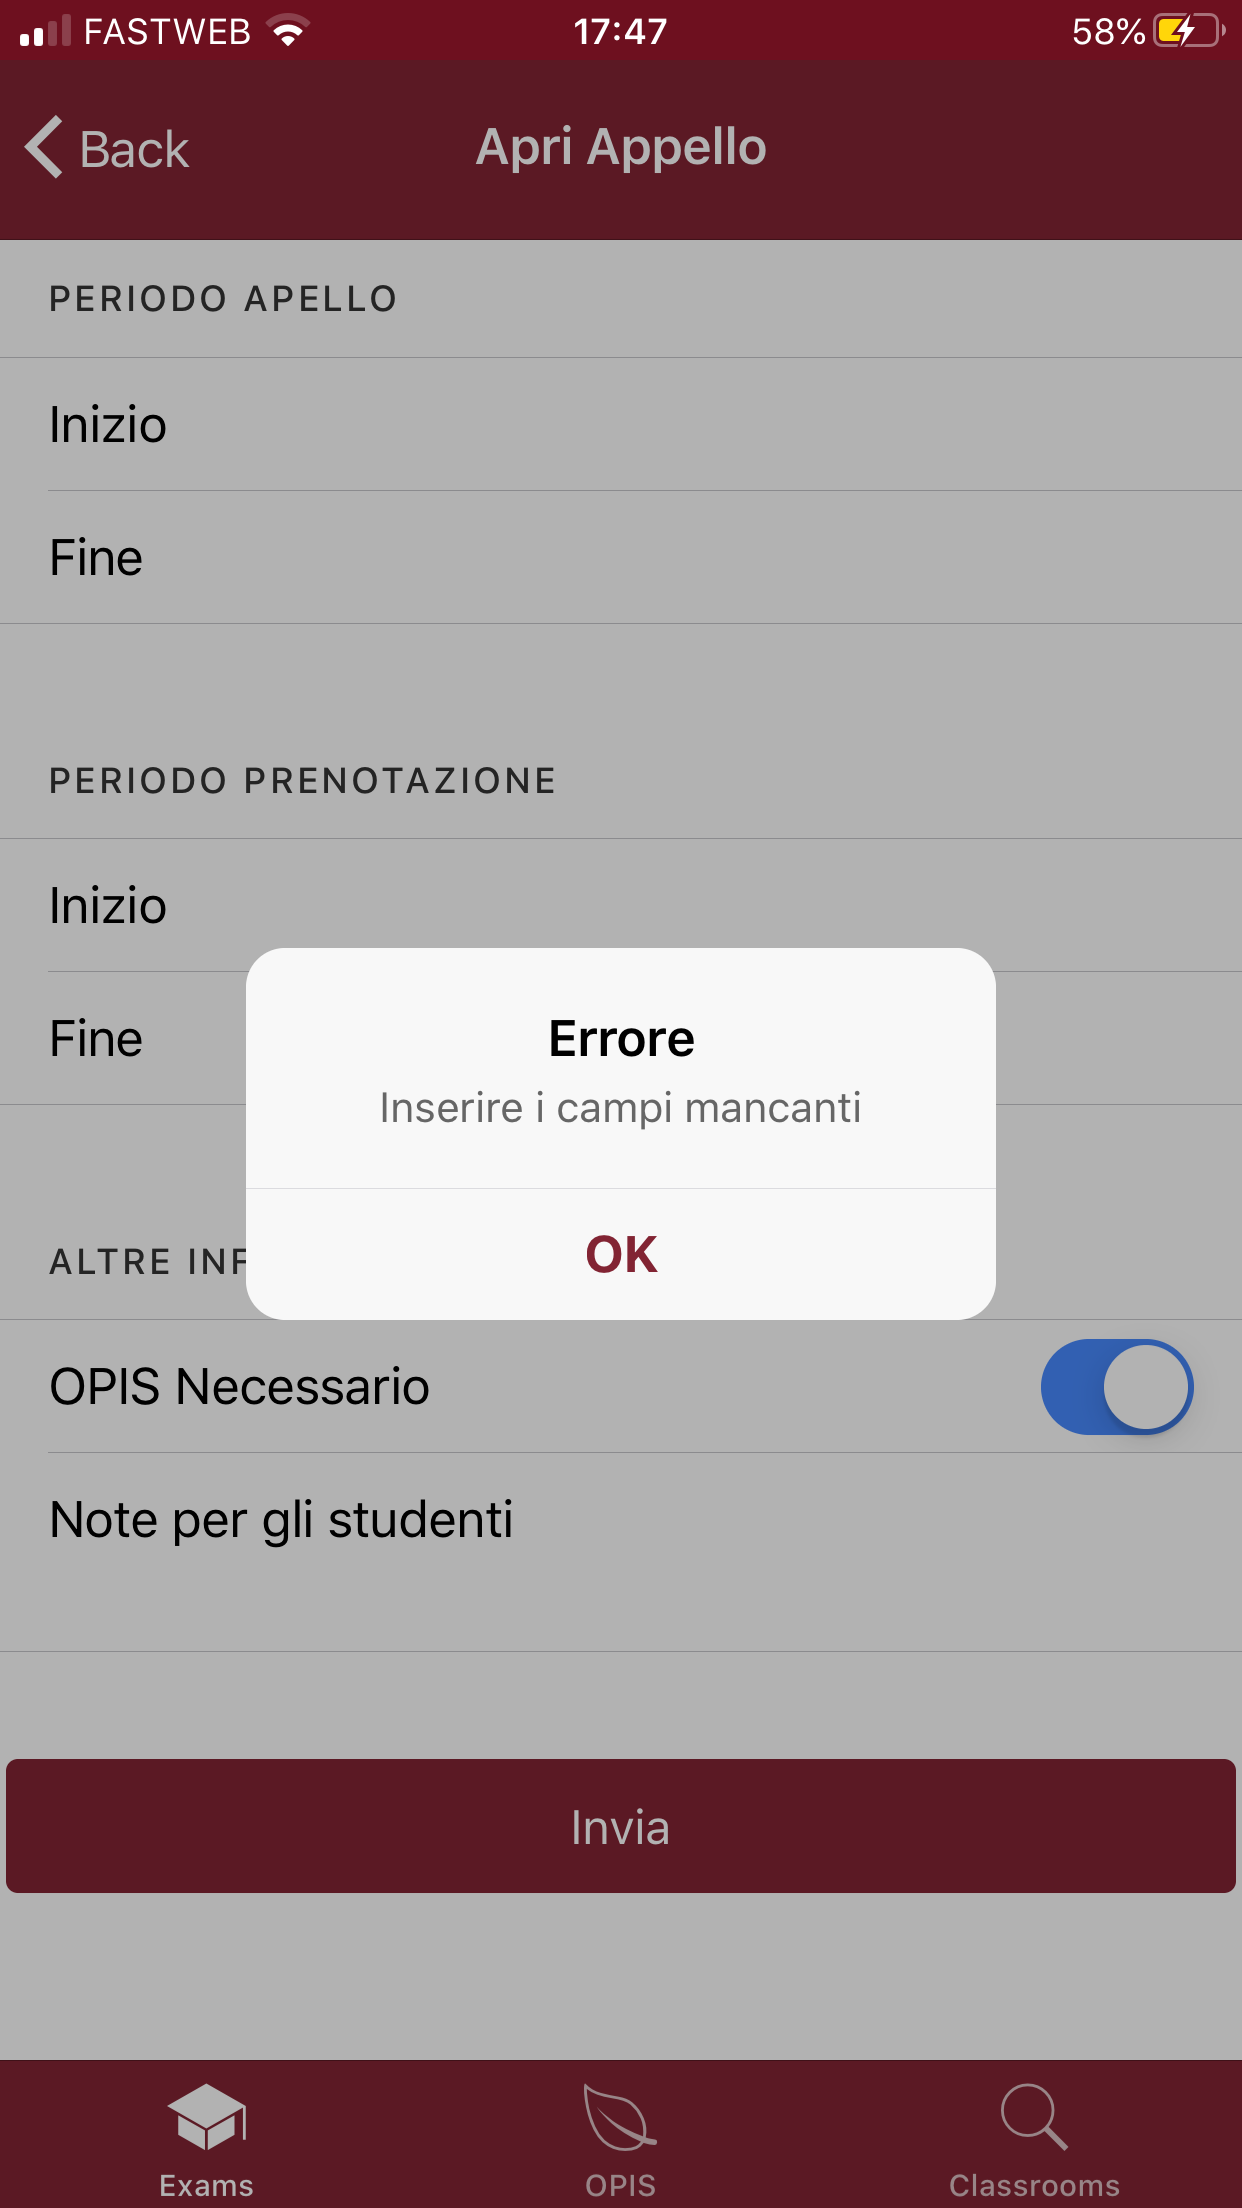
\includegraphics[width=0.5\linewidth]{ui-iterations/i/error-form}  
		\caption{Errore mostrato quando un utente non inserisce tutti i campi.}
		\label{fig:sub-fifth}
	  \end{subfigure}
	  
	\caption{Prototipo della prima iterazione.}
	\label{fig:it-1}
\end{figure}	

\subsection{Iterazione 2}
Il problema più grande dell'iterazione precedente è che la prima view e la seconda (nella quale si inseriscono le date) non sono legate in alcun modo, questo costringe l'utente a ricordare le scelte fatte nella view precedente. Dato che la lista può essere complicata da gestire ed è importante aiutarlo a non fargli commettere errori, ho deciso di cambiare l'ordine della navigazione: la prima pagina infatti è stata spostata all'interno del form, con un bottone "Scegli insegnamenti" che porta alla pagina della scelta degli insegnamenti e degli alias. Quando questi vengono selezionati, si torna indietro e sopra al bottone di prima compaiono gli insegnamenti selezionati.

Altre modifiche all'interfaccia sono state quelle relative ai titoli delle navbar, che ora sono più esplicativi. Sono stati aggiunti dei messaggi di errore e il campo di testo ora è più chiaro ed ha un placeholder. In questa iterazione ho inoltre collegato le view al backend, in modo da lavorare su dei dati che strutturalmente rappresentassero i dati reali. Da qui ho implementato il meccanismo per sintetizzare la tabella degli insegnamenti, in cui parlerò più approfonditamente nella sezione \ref{sec:dev}. Per ora basti sapere che, mentre nell'interfaccia desktop abbiamo almeno due copie per ogni insegnamento (vecchio o presente che sia) \footnote{Gli insegnamenti infatti hanno tutti una voce per l'A.A. corrente e quello precedente.}, nell'app questo non avviene perchè saranno racchiusi in una voce sola. Sarà poi l'app, in modo totalmente trasparente all'utente, a decidere quali corsi e insegnamenti andranno inviati al server.

Anche la grafica è cambiata, rendendola più simile a quella dell'aggiunta di un appuntamento sul calendario di iOS e Google. Non potendo fare più i test di usabilità, che hanno bisogno di essere fatti in presenza, mi sono affidato agli standard che hanno applicazioni più importanti. Infatti l'aggiunta di un appuntamento su un calendario non è tanto differente dall'apertura di un verbale, solo che bisogna gestire tipi differenti di dati.

Infine, invece di utilizzare delle view, ho deciso di usare dei modali per far sparire i tab a fine pagina per impedire all'utente di navigare all'interno dell'applicazione dopo aver iniziato l'apertura di un verbale. Infatti è ragionevole pensare che un esso non voglia farlo, semplicemente perchè ho fatto in modo che tutto ciò che serve gli serve per aprire un verbale è visibile durante la navigazione. In più questo permette di risparmiare un po' di spazio per evitare lo scroll. Nell'immagine \ref{fig:it-2} è possibile vedere tutte le pagine.

Come anticipato ad inizio capitolo \ref{heuristics}, valuterò questa iterazione tramite le euristiche di Neilsen. Possiamo dire che l'interfaccia, arrivata a questo punto, le soddisfa almeno per buona parte.
Per quanto riguarda la prima regola, "Visibilità dello stato del sistema" è soddisfatta da tutti gli elementi tramite dei titoli esplicativi e pulsanti ben visibili. La seconda, "Corrispondenza tra sistema e mondo reale", è soddisfatta pienamente anche lei in quanto i termini "Appello", "Corso", "Insegnamento" e "Facolt\'a" sono gli stessi utilizzati nel gergo comune, inoltre non essendo cambiati dall'iterazione precedente ed avendo fatto dei test su quella, si può assumere che non sia fonte di ambiguità. Anche "Controllo e libertà" viene rispettata tramite l'aggiunta degli alias, che permettono una scorciatoia agli utenti esperti e la scelta dei corsi dà una certa libertà nell'apertura di un appello. L'uniformità dei termini usati garantisce la "consistenza"; mentre la selezione delle date, che deve rispettare determinati vincoli \footnote{Non è possibile selezionare date nel passato e non devono accavallarsi tra di loro.} e sono compilate automaticamente, unita al collasso degli insegnamenti in meno voci all'interno della tabella, garantiscono la prevenzione degli errori, l'efficienza d'uso ed un design minimalista. La regola "riconoscere invece che ricordare" è stata già discussa ad inizio sezione anche se, quando gli alias sono vuoti, non c'è alcuna indicazione su cosa sono e come vengono creati. Per quanto riguarda gli errori, per ora ci sono solo quelli che vengono lanciati quando l'utente preme "ok" senza selezionare una facoltà all'interno dell'alert e quando clicca su "invia" senza aver messo le date e almeno un insegnamento. Come si vede dalle immagini, però, sono stati creati ad arte per essere ben diagnosticabili. Le condizioni per cui un utente può lanciare un errore è solo in questi due casi comunque, quindi sono veramente poche. Vedremo nella terza iterazione come sono riuscito ad abbassare le condizioni a solo un caso, cioè quello dei campi obbligatori mancanti.

\begin{figure}[H]
	\begin{subfigure}{0.6\textwidth}
	  \centering
	  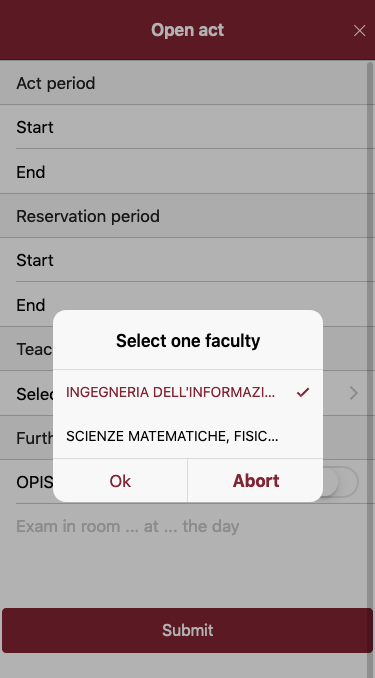
\includegraphics[width=0.5\linewidth]{ui-iterations/ii/select-faculty}  
	  \caption{Alert per la selezione della facoltà.}
	\end{subfigure}
	\begin{subfigure}{0.6\textwidth}
	  \centering
	  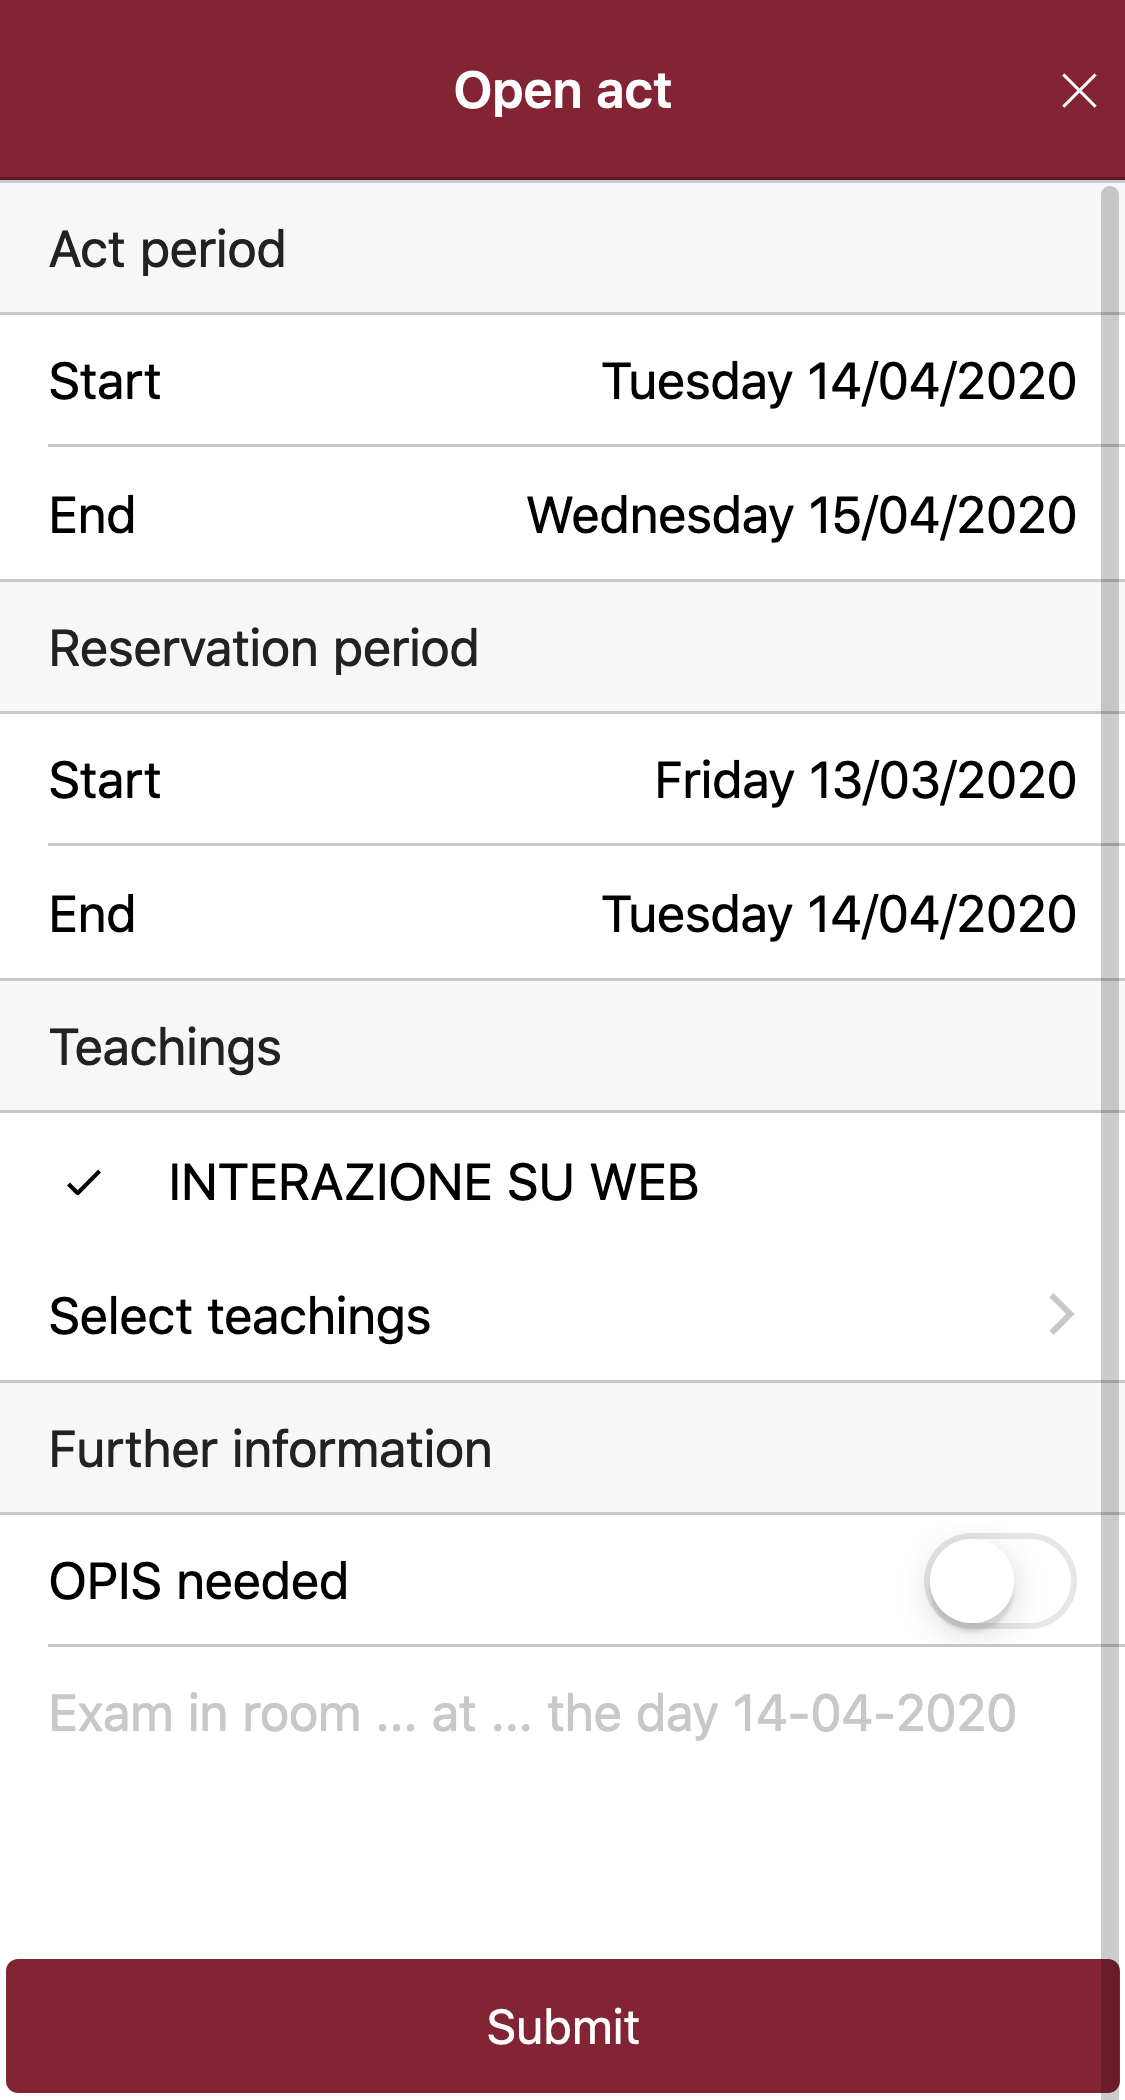
\includegraphics[width=0.5\linewidth]{ui-iterations/ii/form}  
	  \caption{Form con le date inserite ed un inseegnamento selezionato.}
	\end{subfigure}
	\begin{subfigure}{0.6\textwidth}
		\centering
		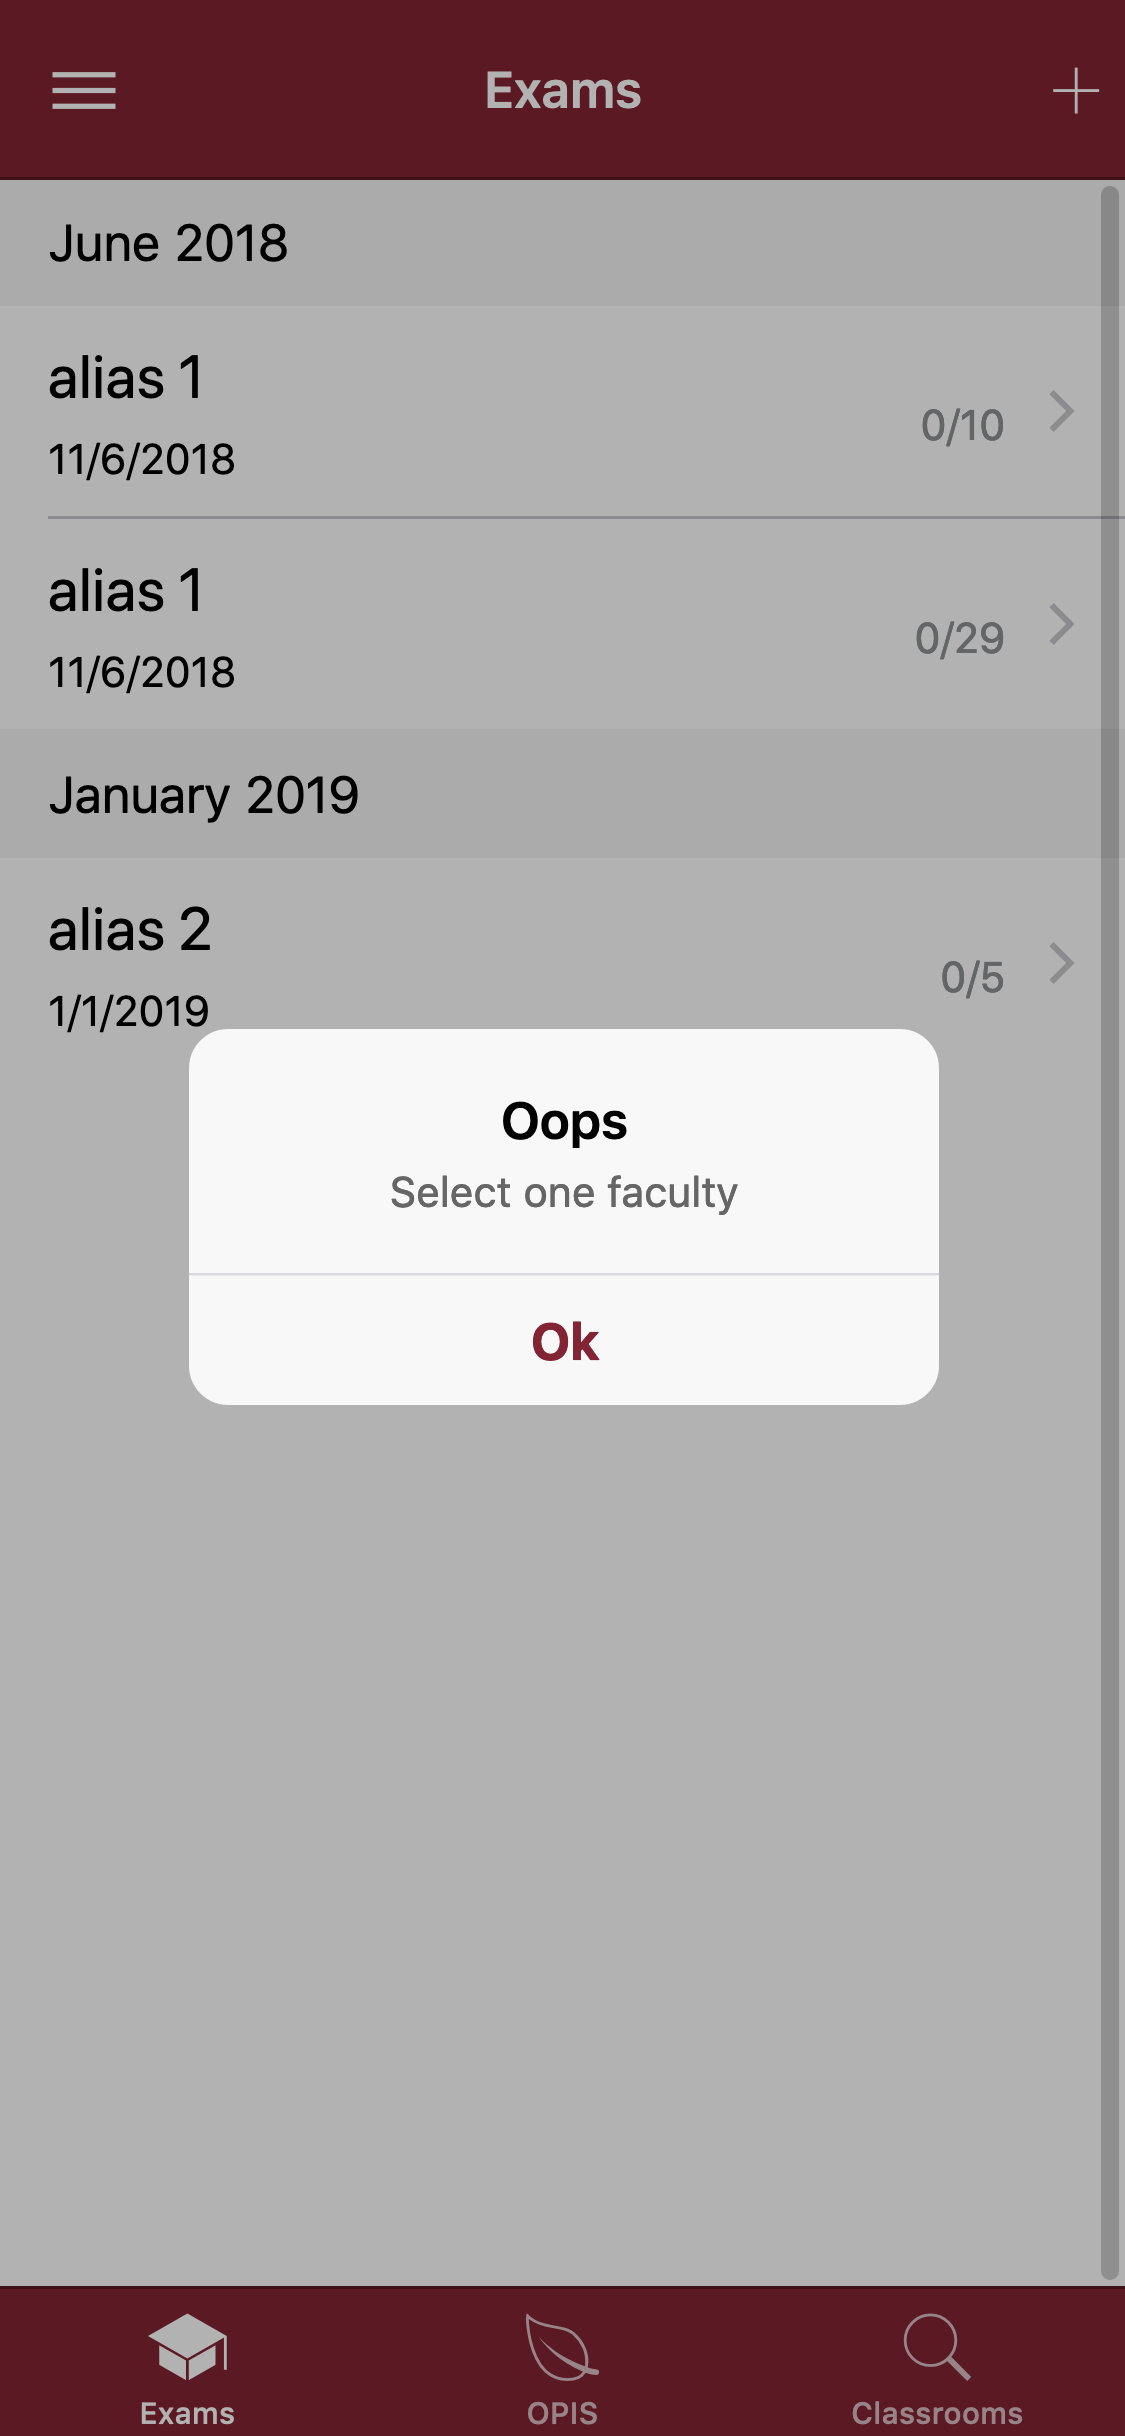
\includegraphics[width=0.5\linewidth]{ui-iterations/ii/error-faculty}  
		\caption{Messaggio di errore.}
	  \end{subfigure}
	  \begin{subfigure}{0.6\textwidth}
		\centering
		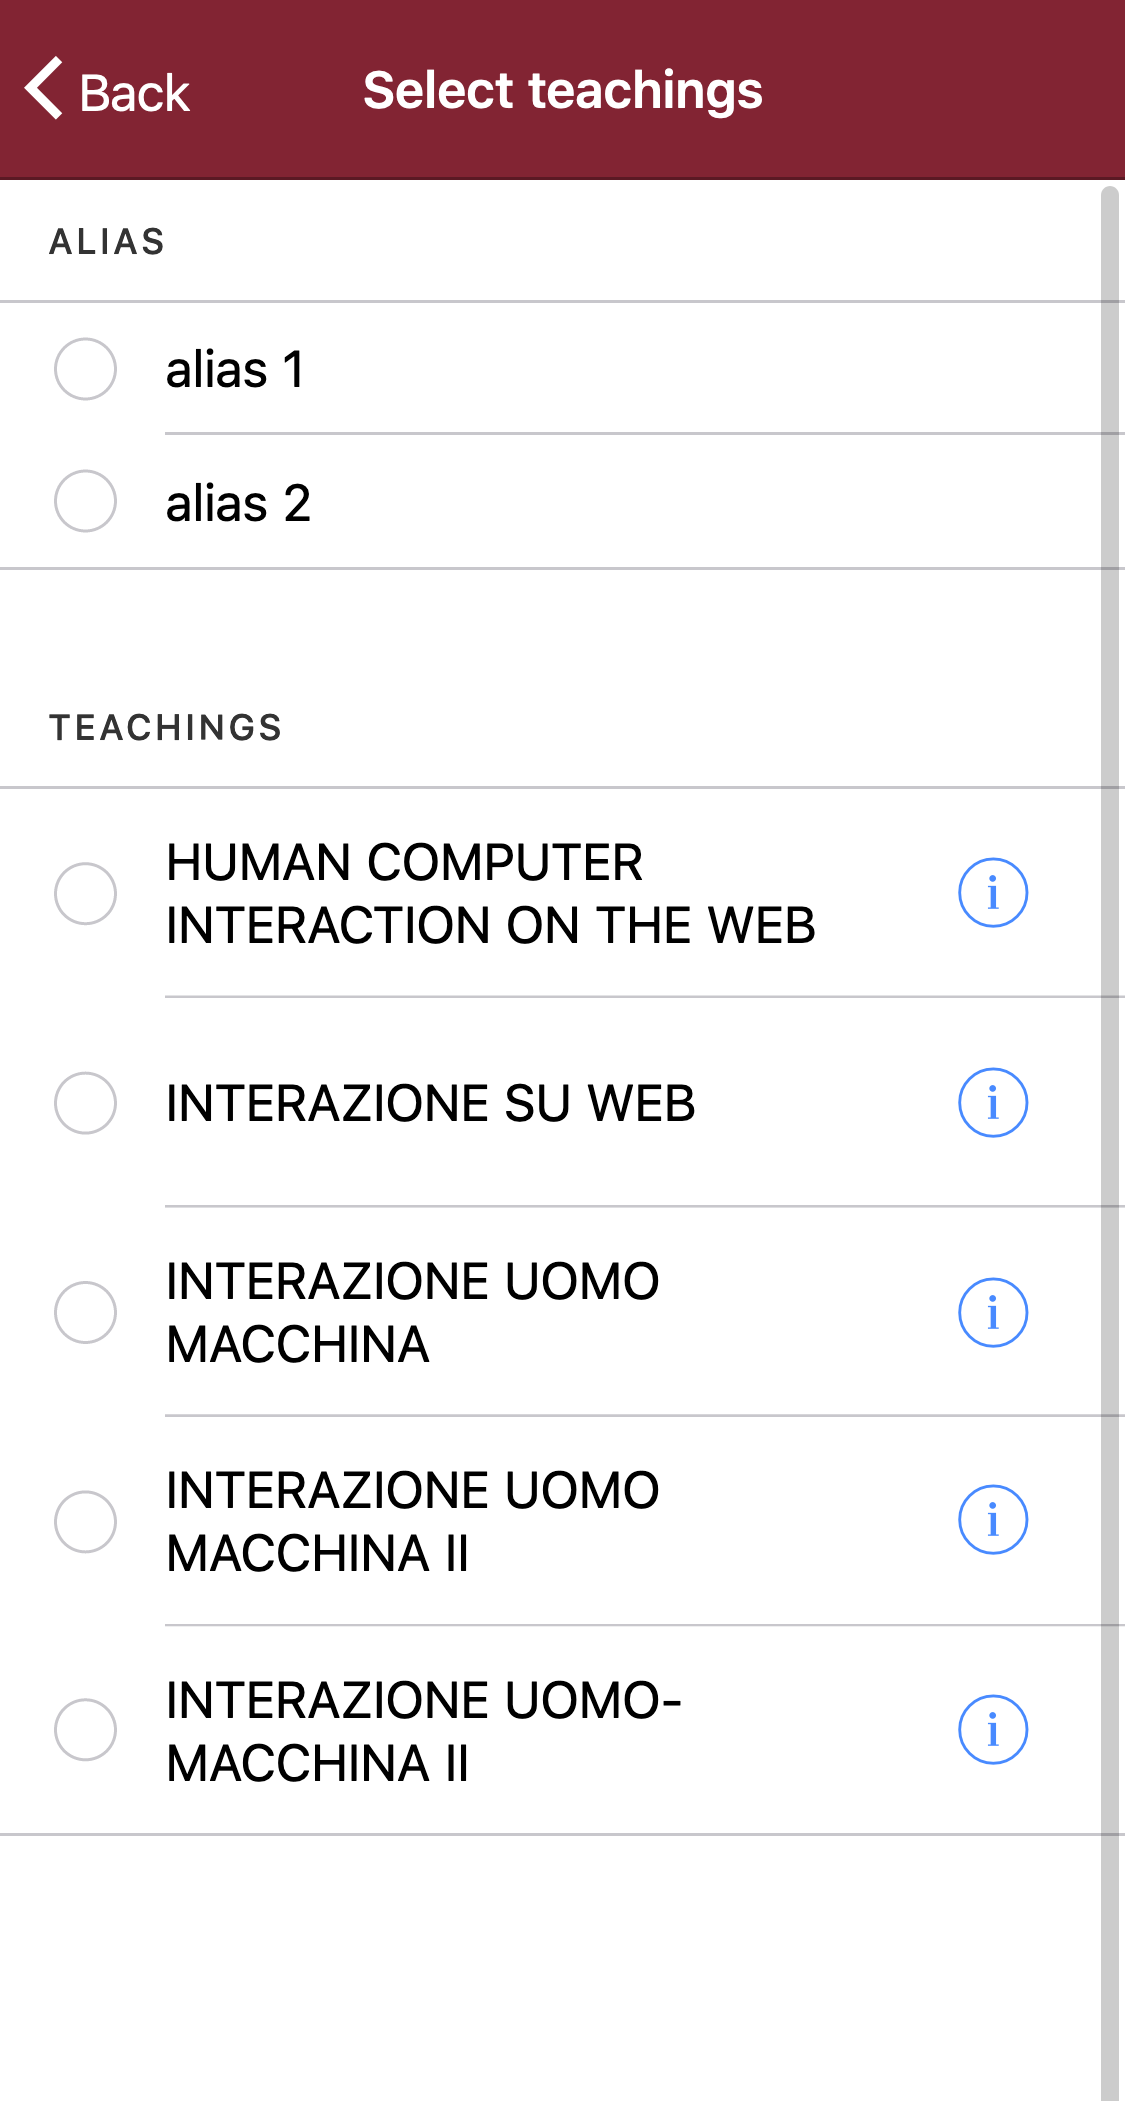
\includegraphics[width=0.5\linewidth]{ui-iterations/ii/teaching-list}  
		\caption{Lista degli insegnamenti.}
	  \end{subfigure}
	  
	\caption{Seconda iterazione.}
	\label{fig:it-2}
\end{figure}

\subsection{Iterazione 3}
La scelta dei corsi di studio è un componente che ho voluto tenere fino ad ora per non togliere libertà di scelta all'utente. Da quanto è emerso nelle interviste e nei test, però, è un elemento che crea confusione e gli utenti sono riluttanti nell'usare tale strumento. Pertanto in questa iterazione abbiamo deciso di oscurare i pulsanti per accedervi e verificare se sia una funzionalità richiesta. Ma se l'ipotesi che non serve fosse corretta allora avremmo tolto una fonte di distrazione e avremmo alleggerito l'interfaccia.

Altri miglioramenti sono stati apportati all'alert per la scelta della facoltà dove ora il bottone per confermare la facoltà è disabilitato finchè non se ne seleziona una (questo elimina un triggher per gli errori). Inoltre le etichette agli input del form sono cambiate, adesso quelle per ogni singolo elemento sono più esplicative e ho tolto i titoli nelle varie sezioni che occupavano solo spazio. Anche il textbox ora è più grigio in modo tale da essere ben visibile all'utente. Infine è stato aggiunto un messaggio che inviti l'utente ad utilizzare gli alias e il perché esistono. Dunque nell'immagine \ref{fig:it-3} si può vedere l'interfaccia finale.

\begin{figure}[H]
	\begin{subfigure}{0.6\textwidth}
	  \centering
	  
\includegraphics[width=0.5\linewidth]{ui-iterations/iii/facolta-1}  
	  \caption{Put your sub-caption here}
	  \label{fig:sub-first}
	\end{subfigure}
	\begin{subfigure}{0.6\textwidth}
	  \centering
	  
\includegraphics[width=0.5\linewidth]{ui-iterations/iii/facolta-2}  
	  \caption{Put your sub-caption here}
	  \label{fig:sub-second}
	\end{subfigure}
	\begin{subfigure}{0.6\textwidth}
		\centering
		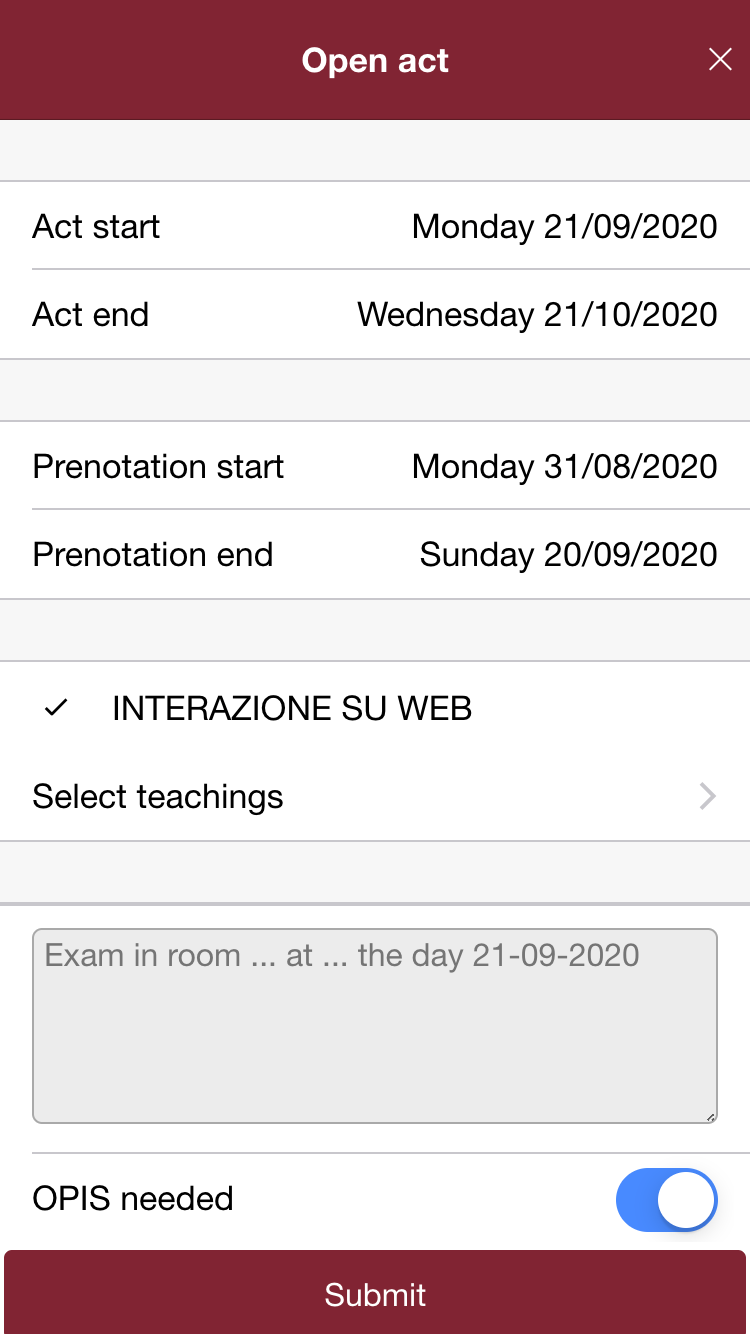
\includegraphics[width=0.5\linewidth]{ui-iterations/iii/form}  
		\caption{Put your sub-caption here}
		\label{fig:sub-second}
	  \end{subfigure}
	  \begin{subfigure}{0.6\textwidth}
		\centering
		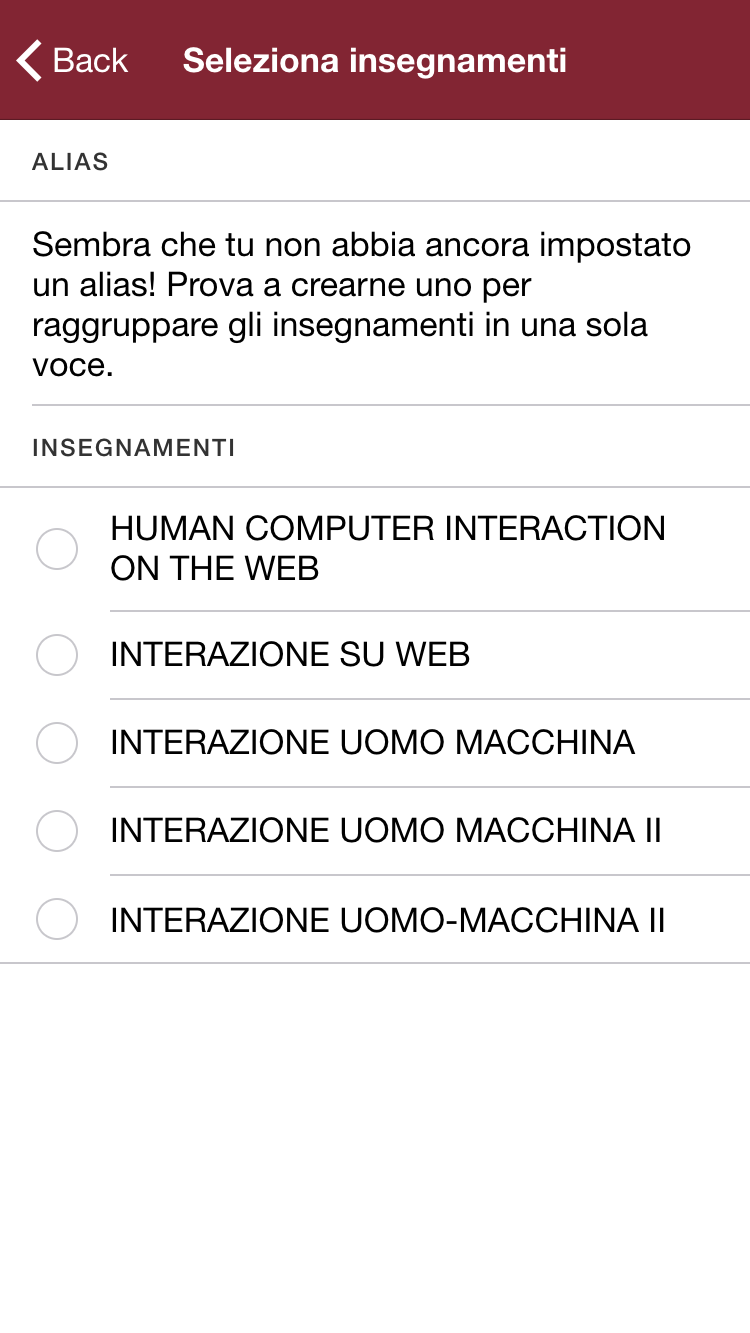
\includegraphics[width=0.5\linewidth]{ui-iterations/iii/insegnamenti}  
		\caption{Put your sub-caption here}
		\label{fig:sub-second}
	  \end{subfigure}
	  
	\caption{Terza iterazione}
	\label{fig:it-3}
\end{figure}

\newpage
\section{Implementazione}
\label{sec:dev}
Spiegate e valutate le idee alla base dell'interfaccia, adesso spiegherò come ho realizzato la funzionalità di apertura di un verbale. In questa sezione andrò più nel dettaglio tecnico di ogni pagina e spiegherò i ruoli che ogni componente ha.

\subsection{Le classi}
Per realizzare tutto ciò che è stato detto nella sezione precedente, ho bisogno delle seguenti classi:
\begin{itemize}
	\item \textbf{ActTeachings}: Rappresenta un appello;
	\item \textbf{Teaching}: Rappresenta un insegnamento;
	\item \textbf{Program}: Rappresenta un corso di studi;
	\item \textbf{Faculty}: Rappresenta una facoltà;
	\item \textbf{ActController}: Ha il compito di raccogliere gli insegnamenti con lo stesso nome in una sola voce;
	\item \textbf{NewActPage}: Rappresenta la UI del form;
	\item \textbf{TeachingListPage}: Mostra la UI per la selezione degli insegnamenti;
	\item \textbf{DetailedListPage}: Mostra la UI per la selezione dei corsi di studio collegati ad un insegnamento;
	\item \textbf{InfoprofProvider}: Classe che accede ai dati del server.
\end{itemize}

Ho dunque realizzato il diagramma delle classi visibile in figura \ref{fig:classDiagram}.
\begin{figure}[H]
	\caption{Diagramma delle classi.}
	\centering
	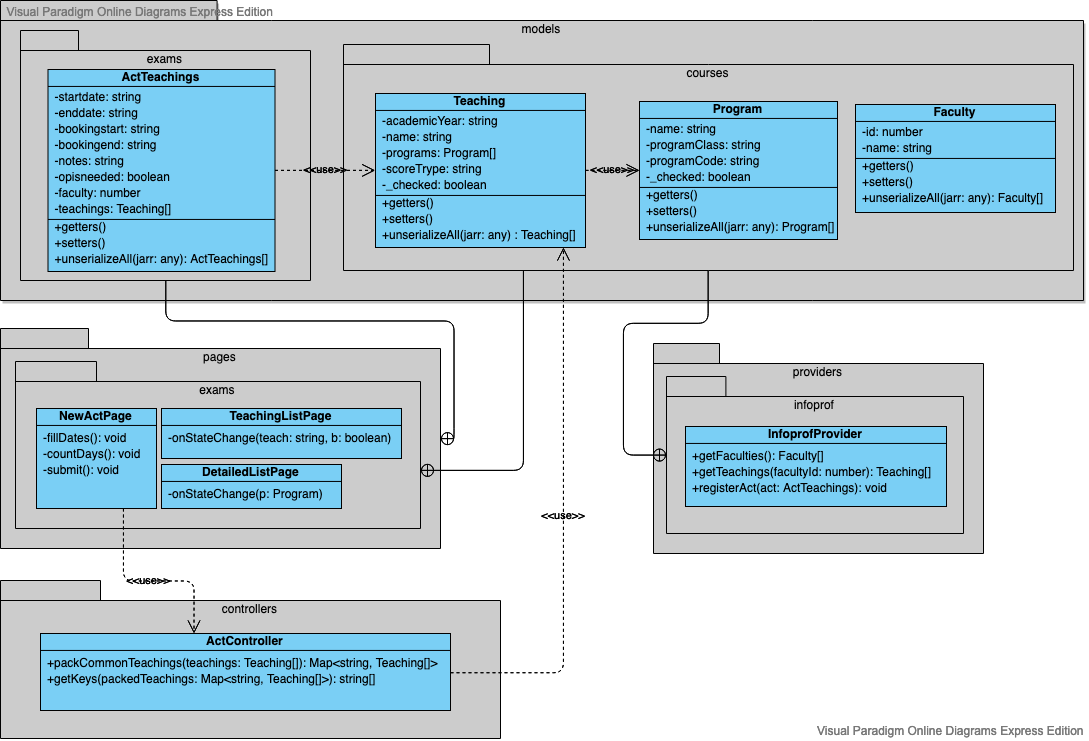
\includegraphics[width=1\textwidth]{diagrams/classDiagram}
	\label{fig:classDiagram}
\end{figure}

\subsection{InfoprofProvider}
InfoprofProvider è la classe che si occupa di utilizzare le API per accedere ai dati nel server, quando questi metodi sono dei "getter" il server risponde con dei dati in formato JSON che andranno deserializzati con gli appositi metodi che ogni classe di tipo "entity" forsnisce nel costruttore o, se trattiamo un array di JSON, allora con il metodo uniserializeAll() fornito sempre dalle classi entity. La funzionalità di apertura di un verbale ha dunque bisogno di comunicare in 2 occasioni con il server, per un totale di 3 chiamate: la prima e la seconda vengono chiamate quando l'utente accede al form di apertura del verbale e scarica prima le facoltà, \textbf{getFaculties()}, in cui l'utente lavora e poi gli insegnamenti corrispondenti alla facoltà scelta, con \textbf{getTeachings()}. L'utlimo metodo, \textbf{registerAct()}, invece viene chiamato quando bisogna registrare l'appello, ovvero quando l'utente clicca sul pulsante "Invia".

\begin{lstlisting}
public registerAct(act: ActTeachings): Promise<void> {
	if (this.professorId == "0000000") {
		return new Promise((resolve, reject) => {
			resolve();
		});
	}
	return new Promise<void>((resolve, reject) => {
		this.http.setDataSerializer("json");
		this.http.put(
			this.env.getInfoprofAPI() + "/acts/",
			act,
			this.getOptions()
		).then(data => {
			this.accessToken = data.headers["x-access-token"] != null ? data.headers["x-access-token"] : this.accessToken;
			console.log(this.accessToken);
			resolve();
		}).catch((err) => this.errorHandler(err, reject));
	});
}
\end{lstlisting}

\begin{lstlisting}
public getFaculties(): Promise<Faculty[]> {
	return new Promise((resolve, reject) => {
		this.http.setDataSerializer("urlencoded");
		this.http.get(
			this.env.getInfoprofAPI() + "/me/acts/faculties/",
			{},
			this.getOptions()
		).then(data => {
			this.accessToken = data.headers["x-access-token"] != null ? data.headers["x-access-token"] : this.accessToken;
			console.log(this.accessToken)
			try {
				resolve(Faculty.unserializeAll(JSON.parse(data.data)));
			} catch (e) {
				console.error("Exception during parse: " + e.toString());
				reject(new ApiError(ApiError.SERVER_ERROR, e.toString()));
			}
		}).catch((err) => this.errorHandler(err, reject));
	});
}
\end{lstlisting}

\subsection{ActController}
\label{sc:controller}
Prima di mostrare come funzionano le pagine è opportuno presentare anche l'ActController che ha il compito di gestire gli insegnamenti in strutture dati diverse dall'array con cui ci vengono dati dal provider. I metodi più importanti sono \textbf{packCommonTeachings()} e \textbf{getKeys()}.

Il primo metodo si occupa di raccogliere tutti gli insegnamenti con lo stesso nome in un dizionario dove le chiavi rappresentano il nome dell'insegnamento e i valori invece sono array contenenti gli insegnamenti che condividono quel nome. Infatti, possiamo vedere che gli appellativi che vengono dati rispettano uno schema: nella prima parte c'è il nome effettivo dell'insegnamento, mentre nella seconda ci sono le informazioni aggiuntive racchiuse tra parentesi. Ecco un esempio \textbf{HUMAN COMPUTER INTERACTION ON THE WEB (cod. 1047630 - INF/01 - cfu: 6, canale: NESSUNA CANALIZZAZIONE)} e \textbf{HUMAN COMPUTER INTERACTION ON THE WEB (cod. 1047630 - INF/01 - cfu: 6, canale: NESSUNA CANALIZZAZIONE)}. Dunque basta tagliare la stringa tra le parentesi per ricavare la chiave e raccogliere tutte le stringhe che matchano con essa in un dizionario.

\begin{lstlisting}
public packCommonTeachings(teachings: Teaching[]): Map<string, Teaching[]> {
	// All teachings with the same names are collected under the same key.
	let map: Map<string, Teaching[]> = new Map<string, Teaching[]>();

	for (let teaching of teachings) {
		let key = teaching.getName().slice(0, teaching.getName().indexOf("(") - 1);
		if (map.has(key)) {
			map.get(key).push(teaching);
		} else {
			let t: Teaching[] = [teaching];
			map.set(key, t);
		}
	}
	return map;
}
\end{lstlisting}

All'interno del DOM è molto complesso lavorare con i dizionari, quindi avere un metodo che all'occorrenza estrae le chiavi in un array e le mostra all'utente è comodo e per questo ho scritto il metodo \textbf{getKeys()}.

\begin{lstlisting}
public getKeys(packedTeachings: Map<string, Teaching[]>): string[] {
	let keys: string[] = [];
	packedTeachings.forEach((value, key) => {
		keys.push(key);
	});
	return keys;
}
\end{lstlisting}

\subsection{NewActPage}
Passando invece alle pagine, NewActPage è la prima in ordine di navigazione e contiene il form nel quale inserire le varie informazioni necessarie al successo dell'operazione. Il primo metodo è \textbf{fillDates()} e, come il nome suggerisce, è il responsabile della compilazione automatica delle date. Il metodo in prima battuta controlla che non ci sia già una data in uno dei campi preposti, apparte actStart. Se la condizione è verificata, si occupa di compilare le date in automatico, altrimenti si ferma per non sovrascrivere quello che l'utente ha fatto in precedenza.
Le variabili \textbf{actPeriod}, \textbf{emptyPeriod} e \textbf{reservationPeriod} rappresentano rispettivamente la differenza espressa in giorni tra la fine dell'appello e l'inizio, l'inizio dell'appello e la fine delle prenotazioni e la fine delle prenotazioni e l'inizio delle stesse (da questo momento chiamerò queste variabili \textbf{periods}). Questi valori vengono presi dallo storage interno del telefono nel del costruttore della classe e assumono "-1" se non esistono valori precedentemente salvati. In quest ultimo caso, la compilazione prenderà dei valori standard che sono un mese per le prenotazioni e l'appello e 1 giorno tra le due.

La seconda parte del metodo si occupa di decidere se le variabili "periods" andranno salvate nello storage. Prima di questo però bisogna tenere presente che ci sono dei vincoli che le date devono rispettare \footnote{Il DOM si occupa di controllare che tutti i vincoli siano soddisfatti.}:
\begin{enumerate}
	\item Il minimo valore che può assumere resStart è "oggi" (chiameto minResStart);
	\item Il minimo valore che può assumere actStart è resStart + 1 giorno (chiamato minActStart);
	\item Il minimo valore che può assumere resEnd è minResStart;
	\item Il massimo valore che può assumere resStart è actStart - 1 giorno (chiamato maxResStart);
	\item Il massimo valore che può asssumere resEnd è  actStart - 1 giorno (chiamato maxResEnd);
\end{enumerate}
A questo punto, se alla fine del calcolo, i valori assunti dalle date violano uno dei vincoli posti, il sistema va ad aggiustare le date interessate in modo che li rispettino tutti. Se si verificasse questa condizione le variabili "periods" assumerebbero valori calcolati dal sistema e non dall'utente, quindi non vanno salvati, ma nello storage rimangono quelli che c'erano precedentemente.

\begin{lstlisting}[frame=single]
private fillDates() {
	if (this.actEnd == undefined && this.resStart == undefined && this.resEnd == undefined) {
		let actStart = moment(this.actStart);
		if (this.actPeriod >= 0) {
			this.actEnd = actStart.add(this.actPeriod, 'd').format("YYYY-MM-DD");
		} else {
			this.actEnd = actStart.add(1, 'M').format("YYYY-MM-DD");
		}
		actStart = moment(this.actStart);
		if (this.emptyPeriod >= 0) {
			this.resEnd = actStart.subtract(this.emptyPeriod, 'd').format("YYYY-MM-DD");
		} else {
			this.resEnd = actStart.subtract(1, 'd').format("YYYY-MM-DD");
		}
		let resEnd = moment(this.resEnd);
		if (this.reservationPeriod >= 0) {
			this.resStart = resEnd.subtract(this.reservationPeriod, 'd').format("YYYY-MM-DD");
		} else {
			this.resStart = actStart.subtract(1, 'M').format("YYYY-MM-DD");
		}

		actStart = moment(this.actStart);
		this.maxResEnd = actStart.subtract(1, "d").format("YYYY-MM-DD");
		this.maxResStart = this.maxResEnd;
		if (moment(this.resStart).isBefore(this.minResStart)) {
			this.resStart = this.minResStart;
			this.savePeriods = false;
		} else if (moment(this.resStart).isAfter(this.maxResStart)) {
			this.resStart = this.maxResStart
			this.savePeriods = false;
		}
		if (moment(this.resEnd).isBefore(this.resStart)) {
			this.resEnd = this.resStart;
			this.savePeriods = false;
		} else if (moment(this.resEnd).isAfter(this.maxResEnd)) {
			this.resEnd = this.maxResEnd;
			this.savePeriods = false;
		}
	}
}
\end{lstlisting}

Questo metodo invece semplicemente calcola le variabili "periods" esattamente come ho spiegato poco sopra.

\begin{lstlisting}
private countDays() {
	let actStart = moment(this.actStart);
	let actEnd = moment(this.actEnd);
	let resStart = moment(this.resStart);
	let resEnd = moment(this.resEnd);
	this.actPeriod = actEnd.diff(actStart, 'd');
	this.reservationPeriod = prenEnd.diff(prenStart, 'd');
	this.emptyPeriod = actStart.diff(prenEnd, 'd');
}
\end{lstlisting}

Infine c'è submit, che viene chiamato quando l'utente clicca sul pulsante "Invia" e si occupa di controllare che tutti i campi obbligatori siano stati riempiti (la correttezza dei dati invece è già verificata a dal DOM). Se lo sono, controlla se si sta aprendo un verbale dopo il 1 gennaio in modo tale da eliminare dalla selezione gli insegnamenti dell'anno accademico passato, poiché non più accettati dal sistema InfoStud desktop. Infine crea un'istanza della classe ActTeachings chiamando il metodo di InfoprofProvider \textbf{registerAct} il quale invia l'appello appena creato al server. Al successo dell'operazione le preferenze sui "periods" vengono salvate nello storage del dispositivo.

\begin{lstlisting}
private submit(isRetryCall?: boolean): void {
	if (this.actStart != undefined && this.actEnd != undefined && this.prenStart != undefined && this.prenEnd != undefined && this.checkedTeachings.length > 0) {
		let loader = this.loadingCtrl.create({
			spinner: 'crescent',
			content: this.txt["RECORD_IN_PROGRESS"],
		});
		loader.present();
		
		// If the start of the act is after the 31-01 of the current academic year, the teachings of the previous
		// academic year will be deselected automatically.
		if (this.actStart > moment(moment().year() + "01" + "31").format("YYYY-MM-DD")) {
			let checkedTeachings = []
			checkedTeachings.push(...this.checkedTeachings)

			for (let t of checkedTeachings) {
				if (t.getAcademicYear().slice(t.getAcademicYear().indexOf("/") + 1) < moment().format("YYYY")) {
					let i = this.checkedTeachings.indexOf(t);
					if (i > -1) {
						this.checkedTeachings.splice(i, 1);
					}
				}
			}
		}

		this.ip.registerAct(
			new ActTeachings({
				"startdate": this.actStart,
				"enddate": this.actEnd,
				"bookingstart": this.prenStart,
				"bookingend": this.prenEnd,
				"notes": this.notes,
				"opisneeded": this.opis,
				"faculty": this.facultyId,
				"teachings": this.checkedTeachings
			})).then(() => {
				// Save the user's preferencies before closing the modal.
				this.countDays();
				this.storage.set("actPeriod", this.actPeriod);
				
				if (this.savePeriods) {
					this.storage.set("reservationPeriod", this.reservationPeriod);
					this.storage.set("emptyPeriod", this.emptyPeriod);
				}
				loader.dismiss();
				this.events.publish('refreshPage');
				this.navCtrl.pop();
			}).catch((error: ApiError) => {
				// Tutte le varie condizioni d'errore, che sono state omesse qui
			});
	} else {
		let alert = this.alertCtrl.create({
			title: this.txt["ERROR"],
			subTitle: this.txt["INSERT_DATES_AND_TEACHINGS"],
			buttons: ['OK']
		});
		alert.present();
	}
}
\end{lstlisting}

\subsection{TeachingListPage}
%spostare questa parte prima di NewActPage
Questa pagina si occupa, per l'appunto, di gestire la grande tabella di ingegnamenti che su InfoStud desktop è il problema più grande di usabilità. Come abbiamo visto nelle sezioni precedenti dedicate alla progettazione della UI, l'intento era di raccogliere tutti quei duplicati che popolavano la tabella. In fondo l'utente, da quel che ho potuto constatare, non è mai interessato a fare distinzioni tra anni accademici, corsi, insegnamenti vecchi che hanno cambiato nome, ecc... Possiamo quindi assumere che la tabella serva solo in casi particolari e quindi ho deciso di sintetizzarla e lasciare che l'app si prenda l'onere di gestire la parte più burocratica, disabilitando anche la selezione dei corsi di studio. All'utente spetterà solo il compito di selezionare per quali insegnamenti l'appello dovrà essere aperto. Per l'appunto ho pensato di raccogliere gli insegnamenti in un dizionario, come visto nella sezione \ref{sc:controller}.

Il metodo \textbf{ionViewWillEnter} fa parte del ciclo di vita di una pagina in Ionic. In sintesi viene chiamato quando la pagina sta per terminare la transizione da quella precedente \cite{ref:ionicViewLifeCycle}. Il compito che ha in questo caso è di far rispettare il seguente vincolo "Un insegnamento è selezionato se e solo se c'è almeno un corso al suo interno che è selezionato", vincolo che su InfoStud desktop non è rispettato. Come è possibile vedere infatti il codice mette a \textit{true} la variabile \textit{b} non appena trova un corso che è "checkato".

\begin{lstlisting}
ionViewWillEnter() {
	this.packedTeachings.forEach((teachings) => {
		let b = false;
		for (let t of teachings) {
			for (let p of t.getPrograms()) {
				if (p.isChecked()) {
					b = true;
				}
			}
			t.setChecked(b);
			this.checked[this.keys.indexOf(t.getName().slice(0, t.getName().indexOf("(") - 1))] = b;
		}
	});
}
\end{lstlisting}

Questo metodo viene chiamato non appena un utente clicca su un insegnamento per selezionarlo. Quello che fa è semplicemente checkare ogni insegnamento, all'interno del dizionario \textit{packedTeachings}, che hanno come chiave \textit{keys} e fa lo stesso con tutti i corsi collegati agli insegnamenti. Inoltre si occupa di gestire gli Alias, che altro non sono che delle stringhe con tutti i nomi completi degli insegnamenti separati da una virgola. Quando all'argomento \textit{teach} viene passato un alias, semplicemente si fa uno split sulla virgola e sulle stringhe risultanti si toglie la parte tra parentesi. A questo punto da \textit{packedTeachings} si ricavano tutti gli insegnamenti collegati alle chiavi. In questo modo, anche se l'input ha due formati differenti, \textit{teach} viene normalizzato in un array \textit{keys} che nel primo caso è composto da un solo elemento, mentre nel caso dell'alias da tanti elementi quanti sono quelli nell'alias.

\begin{lstlisting}
private onStateChange(teach: string, b: boolean) {
	// Check the teachings as 'true' and so ALL the programs contained in
	// the teaching object must be checked as 'true'. If an alias is clicked,
	// then check as 'true' each teaching contained in it and so all the programs.

	let keys = teach.split(", ");		// splits the teachings when coming from an alias
	let teachings: Teaching[] = [];

	for (let k of keys) {
		if (k.indexOf("(") >= 0) {
			k = k.slice(0, k.indexOf("(") - 1);
		}
		if (k.indexOf('Canale') >= 0) {
			continue;
		}
		teachings.push(...this.packedTeachings.get(k.toUpperCase()));
	}

	for (let t of teachings) {
		t.setChecked(b);
		for (let p of t.getPrograms()) {
			p.setChecked(b);
		}
		this.packedTeachings.set(t.getName().slice(0, t.getName().indexOf("(") - 1), teachings);
	}
}
\end{lstlisting}

\subsection{DetailedListPage}
Sebbene questa pagina sia stata disabilitata, non abbiamo scartato il codice in quanto in futuro potrebbe tornare. Probabilmente è la view più semplice, perché di fatto sono le altre a occuparsi di tutto: se immaginiamo la struttura \textit{packedTeachings} come un albero, questa pagina deve preoccuparsi di gestire solo le foglie, cioè i corsi. Saranno poi \textit{TeachingListPage} e \textit{NewActPage} a preoccuparsi di assegnare dei valori true o false agli insegnamenti, come visto nelle sezioni precedenti. Infatti l'unico metodo qui disponibile è \textit{onStateChange()}, che viene attivato dal DOM non appena l'utente clicca su un corso, prendendo come argomento il corso interessato e cambiando il suo valore a true o false.

\begin{lstlisting}
private onStateChange(p: Program) {
	p.isChecked() ? p.setChecked(false) : p.setChecked(true);
}
\end{lstlisting}

\chapter{Conclusioni}
\label{ch:4}

\backmatter
\phantomsection
\begin{thebibliography}{17}

\bibitem{ref:mit}
Tratto da MIT:
\url{http://web.mit.edu/6.813/www/sp18/classes/09-more-learnability/#consistency}

\bibitem{ref:ionicViewLifeCycle}
\url{https://ionicframework.com/docs/angular/lifecycle}

\end{thebibliography}

\end{document}